


\section{Introduction}


Shell models are systems of ordinary differential equations that mimic the mathematical structure of the spectral representation of a partial differential equations \cite{PD2010}. They were introduced in the context of the Navier-Stokes equations to study turbulent cascade dynamics \cite{MHJ,Gledzer1973,Yamada1988a} while avoiding mathematical difficulties inherent in the full nonlinear partial differential equation. We provide a similar treatment of the advection and advection-diffusion equations in the context of transient mixing and use optimization techniques to study shell-model stirring strategies to optimally mix a tracer concentration.

The shell model is designed to show qualitative features of advection, notably conservation of the tracer density variance, i.e., the $L^2$ --- or more precisely $\ell^2$ --- norm of the tracer concentration. Mixing is quantified by a negative Sobolev norm, the $H^{-1}$ norm, for the tracer concentration, with a natural extension to the shell model, that can measure tracer dispersion even in the absence of diffusion. The shell model also displays quantitative correspondence with results for maximal mixing in the partial differential equation formulation including perfect (complete) mixing in finite time for sufficiently weak constraints on the stirring flow field and exponential decay of the mix-norm for other protocols. We extend the optimal stirring analysis to make predictions for the influence of diffusion on mix-norm decay.

This chapter is organized as follows. In Section \ref{sec:ashellmodel} we introduce the shell model. Local- and global-in-time optimization schemes are described in, respectively, Sections \ref{sec:LIT} and \ref{sec:GIT}. The two shell model stirring strategies are compared without diffusion in Section \ref{sec:nondiffusivecase}  and with diffusion in Section \ref{sec:diffusivecase}. The concluding section \ref{sec:discussion_shell} contains a discussion of the results. Appendix \ref{app:shellmodel} contains exact analytical results for a three-shell truncation and derivations of lower bounds on the mix-norm.

%In contrast to previous work,
%Foures {\it et al.}\cite{DF2014} considered controlling the initial velocity field and boundary conditions, for two-dimensional plane Poiseuille flow governed by full Navier-Stokes equations, rather than directly controlling the velocity field. The authors numerically studied the resulting advection and diffusion dynamics of the tracer concentration field due to the induced flow. The authors compared three objectives: optimization of energy, $H^{-1}$ mix-norm, and variance at the final time. They concluded that flows that optimized energy tended to be poor mixers relative to flows obtained by optimizing the $H^{-1}$ mix-norm and variance. 
%
%We are interested in making progress on the following two optimization formulations: 
%\begin{enumerate}
%	\item (Local-in-time optimization) What admissible velocity field produces the best instantaneous mixing rate?
%	That is, what flow field $\mathbf{u}(\mathbf{x}, t)$ realizes
%	\[
%		\min_{\mathbf{u}} \frac{d}{dt} \|\theta(\,\cdot\,,t)\|_{H^{-1}}^{2}
%	\]
%	at each instant of time $t$ subject to the enstrophy or energy intensity constraint. This is the question that Lin {\it et al.} \cite{JFM2011} studied in the partial differential equation setting without diffusion.
%
%	\item (Global-in-time optimization) What time-dependent velocity field will produce the most mixed state at a final time $T$? That is, what flow field $\mathbf{u}(\mathbf{x}, t)$, defined for $t \in [0,T]$, realizes
%	\[
%		\min_{\mathbf{u}}\|\theta(\,\cdot\, , T)\|_{H^{-1}}^{2}
%	\]
%	subject to either a {\it time-average} enstrophy constraint,
%	\[
%		\frac{1}{T}\int_{0}^{T}dt\int_{D}d^{d}\mathbf{x} \, |\nabla \mathbf{u}|^{2}= \frac{L^{d}}{\tau^{2}},
%	\]
%	or a time-average energy constraint,
%	\[
%		\frac{1}{T}\int_{0}^{T}dt\int_{D}d^{d}\mathbf{x} \, |\mathbf{u}|^{2}= U^{2}L^{d}.
%	\]
%\end{enumerate}
%The global-in-time optimization constraints allow the option of using the budget in a non-uniform fashion in time.  Global-in-time optimization, a full optimal control problem as formulated here, is still an open challenge with partial results provided by Mathew {\it et al.} \cite{Mathew2007b} and Cortellezi {\it et al.} \cite{Cortelezzi2008}. The proposed shell model agrees with the local-in-time optimization results at a qualitative level and provides new insights into the global-in-time optimization problem which will be the focus of future work. 
%

\section{A shell model}
\label{sec:ashellmodel}
Shell models are coarse-grain versions of the spectral representation of a partial differential equation. In particular the Fourier transform of the advection-diffusion equation (\ref{eq:PDE_advection}) becomes the infinite set of coupled ordinary differential equations
\begin{equation*}
	\partial_{t}\hat{\theta}(\mathbf{k},t)+i\sum_{j= 1,2,3}\sum_{\mathbf{k}'\in K}\hat{u}_{j}(\mathbf{k}-\mathbf{k}',t) \, k'_{j} \, \hat{\theta}(\mathbf{k}',t)+ \kappa \, |\mathbf{k}|^2\hat{\theta}(\mathbf{k},t)=0.
\end{equation*}


We course-grain this relation by `binning' the Fourier variables $\hat{\theta}(\mathbf{k},t)$ with wavenumbers $2^{n-1} k_{0}<|\mathbf{k}|<2^n k_{0} $ ($k_{0} = \frac{1}{2L}$) into a single variable $\theta_{n}(t)$ for $n=1,2, \dots ,\infty$. This binning process divides $\mathbf{k}$-space into concentric shells and hence the name---shell model. We similarly course-grain the Fourier amplitudes of the flow field $\hat{u}_{i}(\mathbf{k},t)$ into the variables $u_{n}(t)$ and look for the simplest shell model that retains mode-coupling between neighboring shells.
Thus, we choose the following form:
\begin{equation}
	\label{eq:shellNN_advection}
	\frac{d}{dt} \theta_{n}= k_{n-1}u_{n-1}\theta_{n-1}-k_{n}u_{n}\theta_{n+1} - \kappa \,  k_{n}^{2} \theta_{n}, \quad n=1,2,\dots,
\end{equation}
where $k_{n}=k_{0}2^{n}$ and $\theta_{0} \equiv 0 \equiv u_{0}$. $\kappa$ has units of $L^{2}/T$; $k_{n}$ has units of $1/L$; $u_{n}$ has units of $L/T$; and $\theta_{n}$ is unitless.
We may also consider $N$-shell truncated models with $n=1,2,\dots, N$ where $\theta_{n \ge N+1} = 0 = u_{n \ge N}$. See references \cite{MHJ,wirth1996,PD2010} for alternative shell models of advection-diffusion. 

This construction is not intended to be mathematically rigorous. Rather, it is meant to mimic the natural cascade of the spectrum of the tracer, progressively visiting each shell as stirring stimulates smaller length scales. Note that this model preserves the relation $\frac{d}{dt}\ltwo{\theta}^2 = -2\kappa \hone{\theta}^2$ (found by multiplying the advection-diffusion equation by $\theta$ and integrating over $D$), but now in an $l^{2}$ sense:
\begin{equation}
	\label{eq:shell_L2decay}
	\frac{d}{dt}\sum_{n=1}^{}\theta_{n}^2=- 2\kappa \sum_{n=1}^{}k_{n}^2\theta_{n}^2.
\end{equation}
It follows that the $l^{2}$ norm is conserved for the non-diffusive case.

Lastly, we define the $h^{\alpha}$ shell-model Sobolev norm as
\begin{equation}
	\|\psi(t)\|^2_{h^{\alpha}} \equiv \sum_{m=1}^{} k_{m}^{2\alpha}\psi^{2}_{m}(t).
\end{equation}
for any vector $\psi = (\psi_{1}, \psi_{1}, \dots)$. The shell-model $h^{-1}$ mix-norm is defined as $\| \theta (t) \|_{h^{-1}}$. We denote the intensity constraints of the shell-model flow in terms of $\| u (t) \|^{2}_{h^{\alpha}}$. When $\alpha=0$ this is the $\ell^2$ analog of the energy and $\alpha=1$ returns an expression for enstrophy. The norm operator  $\|\cdot\|_{h^{\alpha}}$ has units of $L^{-\alpha}$.

\section{Instantaneous optimization}
\label{sec:LIT}

We begin by asking, ``What admissible control will produce the best instantaneous mixing rate?'' The analysis shown here parallels the work done by Lin {\it et al} \cite{JFM2011} in the partial differential equation setting. We formulate this question as the following: find the $u$ that realizes
\begin{equation}
	\label{eq:shellNN_lit_prob}
	\min_{u}  \frac{d}{dt} \| \theta (t) \|^{2}_{h^{-1}}
\end{equation} at each time $t$ subject to the constraint
\begin{equation}
	\label{eq:shellNN_lit_contstraint}
	\| u (t) \|_{h^{\alpha}} =W^{(\alpha)}
\end{equation}
where $W^{(0)}=U$ (energy) and $W^{(1)}=1/\tau$ (enstrophy). The root-mean-square rate-of-strain $\Gamma$ is given by $\Gamma = 1/\tau$.

Differentiating the mix-norm and using (\ref{eq:shellNN_advection}), we find
\begin{equation}
	\label{eq:deriv_mix_norm}
	\frac{d}{dt} \| \theta (t) \|^{2}_{h^{-1}} = 2 \sum_{n=1}  \left(k_{n+1}^{-2}-k_{n}^{-2}\right)\theta_{n}\theta_{n+1}k_{n}u_{n} - \kappa \,  \theta_n^2
\end{equation}
and the optimization problem is solved by the method of Lagrange multipliers. The solution is
\begin{equation}
	\label{eq:LIT_optimal}
	u_{n}^{(\alpha)}(t) =-\frac{W^{(\alpha)}\gamma^{(\alpha)}_{n}(t)}{k^{\alpha}_{n}\|\gamma^{(\alpha)}(t)\|_{l^{2}}}
\end{equation}
where $ \gamma^{(\alpha)}_{n}(t) \equiv (k_{n+1}^{-2}-k_{n}^{-2})k_{n}^{1-\alpha} \, \theta_{n}(t) \, \theta_{n+1}(t)$ --- at least, when $\|\gamma^{(\alpha)}(t)\|_{l^{2}} \neq 0$.

An alternative stategy is needed when $\|\gamma^{(\alpha)}(t)\|_{l^{2}} = 0$. An analgous situation arises in the partial differential equation setting \cite{JFM2011} and the second derivative $ \frac{d^{2}}{dt^2} \| \theta (t) \|^{2}_{h^{-1}} $ is minimized instead at these instances. We will do the same here. We write the second derivative as
\begin{equation}
	\label{eq:LIT_2derivative}
	\frac{d^{2}}{dt^2} \| \theta (t) \|^{2}_{h^{-1}} =u^{T}Bu+c^{T}u+d
\end{equation}
where
\[
	B_{nm}\equiv\left\{
	\begin{array}{cl}
		2(k_{n+1}^{-2}-k_{n}^{-2})k_{n}^{2}(\theta_{n}^{2}-\theta_{n+1}^{2}) & m=n              \\
		-2(k_{n+1}^{-2}-k_{n}^{-2})k_{n}k_{n+1}\theta_{n}\theta_{n+2}        & m=n+1            \\
		2(k_{n+1}^{-2}-k_{n}^{-2})k_{n}k_{n-1}\theta_{n-1}\theta_{n+1}       & m=n-1            \\
		0                                                                    & \mbox{otherwise}
	\end{array}
	\right. ,
\]
\[
	c_{n} = -2\kappa \, (k^{-2}_{n+1}-k^{-2}_{n})(k_{n+1}^{2}+k_{n}^{2})k_{n}\theta_{n}\theta_{n+1} ,
	\qquad \text{ and } \qquad
	d=\sum_{n=1} 4 \kappa^2 \, k_{n}^{2}\theta_{n}^{2}.
\]
We want to find the minimum of (\ref{eq:LIT_2derivative}) subject to the intensity constraint (\ref{eq:shellNN_lit_contstraint}).
By the method of Lagrange multipliers, the optimizer satisfies the following system of equations:
\begin{IEEEeqnarray}{rCl}
	\label{eq:system_of_equations}
	\left(B^{T}+B-\lambda K^{(\alpha)} \right) \,u & = & -c \IEEEyesnumber\IEEEyessubnumber* \\
	\|u\|_{h^{\alpha}}& = &  W^{(\alpha)}
\end{IEEEeqnarray}
where $\lambda$ is a lagrange multiplier and $K^{(\alpha)}=\mbox{diag}(k_{1}^{2\alpha}, \dots, k_{N-1}^{2\alpha})$. The general local-in-time strategy is to minimize the $(n+1)$th time derivative of $\|\theta(t)\|_{h^{-1}}$ if the control $u$ does not affect the $1$st through $n$th derivatives. We will soon return to the local-in-time strategy when applying it in sections \ref{sec:nondiffusivecase} and \ref{sec:diffusivecase}.

\section{Global-in-time optimization}
\label{sec:GIT}
Let's explore the global-in-time strategy which optimizes mixing at the end time rather than instantaneously. In this case we wish to solve the following global-in-time optimization problem: at some final time $T > 0$ find
\begin{equation}
	\label{eq:shellNN_git_probM}
	\min_{u}  \| \theta (T) \|^{2}_{h^{-1}} 
\end{equation}
subject to the time averaged intensity constraint
$
\frac{1}{T}\int_{0}^{T}\| u (t) \|^{2}_{h^{\alpha}}\: dt = [W^{(\alpha)}]^2.
$
Toward this end we introduce the augmented Lagrangian
\begin{multline*}
	\mathcal{ L} \{ \theta, u,\phi,\mu \} = \frac{1}{2} \sum_{n=1}^{}\frac{\theta_{n}^{2}(T)}{k_{n}^2} + \int_{0}^{T}\Bigg \{\sum_{n=1}^{}\phi_{n}\left(k_{n-1}u_{n-1}\theta_{n-1}-k_{n}u_{n} \theta_{n+1}- \kappa k_n^2 \theta_n -\dot{\theta}_{n}\right) \\
	+  \frac{\mu }{2}\left( \sum_{n=1}^{}k_{n}^{2\alpha}u_{n}^{2} - [W^{(\alpha)}]^2\right)  \Bigg\}\: dt
\end{multline*}
where for truncated shell models the first two sums above run up to $n=N$ while the third terminates at $N-1$. At extrema the first variations vanish with respect to the variables $\theta, \phi, u$ and $\mu$:

\begin{subequations}
	\label{eq:first_variation}
	\begin{align}
		\frac{\delta \mathcal{L}}{\delta \theta_{n}(T)}&=0  \Rightarrow & \frac{\theta_{n}(T)}{k_{n}^2}-\phi_{n}(T)&=0
		\label{eq:first_variation_terminal} \\
		\frac{\delta \mathcal{L}}{\delta \theta_{n}}&=0  \Rightarrow  & \dot{\phi}_{n}- k_{n-1}u_{n-1}\phi_{n-1} + k_{n}u_{n} \phi_{n+1} - \kappa \, k_n^2\phi_n &=0
		\label{eq:first_variation_adjoint} \\
		\frac{\delta \mathcal{L}}{\delta \phi_{n}}&=0  \Rightarrow  & \dot{\theta}_{n}- k_{n-1}u_{n-1}\theta_{n-1} + k_{n}u_{n} \theta_{n+1} + \kappa \, k_n^2\theta_n &=0
		\label{eq:first_variation_state} \\
		\frac{\delta \mathcal{L}}{\delta u_{n}}&=0 \Rightarrow  &  k_{n}\phi_{n+1}\theta_{n} - k_{n}\phi_{n}\theta_{n+1}+\mu k_{n}^{2\alpha}u_{n} &=0
		\label{eq:first_variation_optimality} \\
		\frac{\delta \mathcal{L}}{\delta \mu}&=0 \Rightarrow &
		\frac{1}{T}\int_{0}^{T}\| u (t) \|^{2}_{h^{\alpha}}\: dt - [W^{(\alpha)}]^2 &= 0
		\label{eq:first_variation_constraint}
	\end{align}
\end{subequations}
Thus, (\ref{eq:first_variation}) holds true for all extrema of the augmented Lagrangian and therefore gives necessary conditions for a global optimizer. 


 For the non-diffusive case, an explicit calculation of the time derivative of $\| u(t)\|_{h^{\alpha}}$ reveals that $\| u(t)\|_{h^{\alpha}}$ is conserved for an optimal trajectory by making use of (\ref{eq:first_variation}) as done in Appendix \ref{appendix:budget_conservation}. This is interesting, since we only demanded that the {\it time-average} of stirring strength be fixed and equal to $W^{(\alpha)}$. An analogous statement holds in the context of the partial differential equation as well (see Chapter \ref{chap:git}) which is an extension of the results first demonstrated by Mathew {\it et al} \cite{Mathew2007b}. The theory developed here will be applied to various cases in the next two sections.


\section{Mixing without diffusion}
\label{sec:nondiffusivecase}

We will first consider the local-in-time strategy starting from the most unmixed state. Then we study the three-shell truncated model which demonstrates the difference between local-in-time and global-in-time strategies. Lastly before introducing diffusion, we will show that the key features of global-in-time optimization shown in three-shell truncated model carry over naturally to models with a larger number of shells.

\subsection{Local-in-time strategy for infinite system}
\label{sec:LIT_MUIC}


Consider the enstrophy-constrained case and start the infinite system with the most unmixed possible state, $\theta(0)=(1, 0 , 0 \dots)^{T}$.  The local-in-time strategy uses each component of the control vector $u$ sequentially and in a piecewise fashion over time. We segment time into intervals, $[t_{n},t_{n+1}]$, of equal duration where $t_{n}= \frac{ \tau (n-1) \pi }{2} $ is the time when the state vector is entirely in the $n$th shell ($\theta_n =1$ and $\theta_{m\neq n}=0$). More precisely for $t\in
[t_{n},t_{n+1}]$, the optimal control is  $u_{n}= \frac{1}{\tau k_{n}}$ and $u_{m\neq n} =0$ while the state vector is given by $\theta_{n}(t) =\cos ((t - t_{n})/\tau)$ and $\theta_{n+1}(t) = \sin ((t - t_{n})/\tau) $ and all other components of $\theta$ are identically zero. The local-in-time strategy is shown graphically in figure \ref{fig:lit_muic}. We find that the mix-norm evaluated at times $t_{n}$ falls off exponentially;  Given that $\| \theta (t_{n}) \|^{2}_{h^{-1}}=\frac{1}{2 k_{n}^{2}}=\frac{1}{2  \, 2^{2n-2}}$ and using the relation $t_{n}= \frac{ \tau (n-1) \pi }{2} $ , we find that
\begin{equation}
	\| \theta (t_{n}) \|_{h^{-1}}=\| \theta (0) \|_{h^{-1}}\exp(- \log(2) t_{n} /\pi \tau).
\end{equation}
We highlight that this exponential decay agrees qualitatively with known results on the mixing rate with the enstrophy constraint \cite{GI2014,CS2013,JFM2011,Alberti2014a, Yao2014a}. In fact it can be shown definitively that the mix-norm decays no faster than exponentially. More precisely, (see Appendix \ref{appendix:lower_bound_enstorphy_nodiff} for derivation)
\begin{equation}
	\label{eq:bound_enstrophy_no_diff_main_text}
	\| \theta (t) \|_{h^{-1}} \geq \|\theta (0)\|_{h^{-1}} \exp \left( - \frac{3t}{2\tau} \right)
\end{equation}
for {\it every} stirring strategy.
The local-in-time strategy is illustrated in figure \ref{fig:lit_muic} and compared to this bound (\ref{eq:bound_enstrophy_no_diff_main_text}).

For the energy-constrained case, we again segment time into intervals $[t_{n},t_{n+1}]$ which are geometrically decreasing in duration where the times  $t_{n}$ are defined by $t_{n+1}= t_{n}+\Delta t_{n}$, $t_{1}=0$, and $\Delta t_{n}= \frac{ \pi }{2Uk _{n}} $. During each interval $[t_{n},t_{n+1}]$, the control is given by $u_{n}= U$ and $u_{m\neq n} = 0$ while the state vector is given by $\theta_{n}(t) =\cos (k_{n} U (t - t_{n}))$ and $\theta_{n+1}(t) = \sin (k_{n} U (t - t_{n})) $. Therefore the solution is similar to the enstrophy-constrained case except now the intervals are shrinking at a geometric rate. Thus the mix-norm goes to zero ($\lim_{n\rightarrow \infty} \| \theta (t_{n}) \|_{h^{-1}}= \lim_{n\rightarrow \infty} \frac{1}{k_{n}} =0$) in finite time since
\begin{equation}
	(t_{\infty}\equiv) \lim_{n \rightarrow \infty} t_{n} = \sum_{n=1}^{\infty} \Delta \tau_{n} =  \frac{ \pi }{2k_{0} U}.
\end{equation}
Note that if the entire concentration starts in the $m$th shell ($\theta(0)=\mathbf{e}_{m}$), then $t_{\infty}$ becomes the partial sum $t_{\infty}=\sum_{n=m}^{\infty}\Delta \tau_{n}$.  Once more we get qualitative agreement with known results from fluid mixing. Lunasin {\it et al} \cite{JMP2012} showed that perfect mixing in finite time for a simple binary distribution with fixed energy is indeed possible. 

We also obtain a lower bound for the energy-constrained case: (see derivation in Appendix \ref{appendix:bound_energy_no_diff})
\begin{equation}
	\label{eq:bound_energy_no_diff_main_text}
	\|\theta (t) \|_{h^{-1}} \geq\|\theta (0) \|_{h^{-1}}(1 -t/t_c)
\end{equation}
where $t_{c}=\frac{2}{3U}\frac{\|\theta(0)\|_{h^{-1}}}{\|\theta (0) \|_{l^{2}}}$. Figure \ref{fig:lit_muic} shows the local-in-time strategy for this case compared to the bound (\ref{eq:bound_energy_no_diff_main_text}) shown above.

In either constraint, the state vector moves from plane to plane. The state vector first rotates in the $\theta_{1}$-$\theta_{2}$ plane from the $\theta_{1}$ axis to the $\theta_{2}$ axis and then rotates in the $\theta_{2}$-$\theta_{3}$ plane from the $\theta_{2}$ axis to the $\theta_{3}$ axis and so forth. Note that for this particular initial condition, the analysis holds for $N$-shell truncated models and the above strategy holds for times $t < t_{N}$. When $t=t_{N}$, the state vector has reached the final shell and it is no longer possible to decrease the mix-norm any further.  Note that the local-in-time strategy behaves somewhat like a discrete analog to the self-similar strategies \cite{Alberti2014a,Yao2014a} found in the continuous partial differential equation problem since the same transformation is applied sequentially at piecewise time intervals at smaller and smaller scales.


\begin{figure*}[!ht]
	\centering
	\includegraphics[width=1.0\textwidth]{ch-shellmodel/images/lit_muic}
	\caption{Local-in-time strategy without diffusion starting initially from the most unmixed state. The entrophy-constrained case ($\frac{1}{\tau}=1$) is shown on the left subplots where (A) shows the state, (B) shows the control, and (C) shows the mix-norm. The energy-constrained case ($U=1$) is shown on the right subplots where (D) shows the state, (E) shows the control, and (F) shows the mix-norm. }
	\label{fig:lit_muic}
\end{figure*}



\subsection{Global-in-time strategy for 3-shell truncated model with enstrophy constraint}
\label{sec:git_enstrophy_3shell}

The diffusionless 3-shell truncated model, given by 
\begin{equation}
	\label{eq:3_mode_state}
	\left(
	\begin{array}{c}
		\dot{\theta}_{1} \\
		\dot{\theta}_{2} \\
		\dot{\theta}_{3}
	\end{array}
	\right)
	=\underbrace{ \left(
		\begin{array}{ccc}
			0          & -k_{1}u_1 & 0         \\
			k_{1}u_{1} & 0         & -k_{2}u_2 \\
			0          & k_{2}u_2  & 0
		\end{array}
		\right)}_{\equiv A(t)}
\left(
\begin{array}{c}
	\theta_{1} \\
	\theta_{2} \\
	\theta_{3}
\end{array}
\right),
\end{equation}
is the simplest reduced model that retains many interesting features of the full infinite system. From the last section, we know that the local-in-time strategy is to move along planes one by one. This holds for the 3-shell truncated model as well. 

Now, let us determine how you can improve upon the local-in-time strategy by considering the global-in-time strategy. We would like to minimize
$\| \theta (T) \|^{2}_{h^{-1}}$ subject to the enstrophy constraint, $\frac{1}{T}\int_{0}^{T}\| u(t)\|^{2}_{h^{1}} dt =  \frac{1}{\tau^2}.$ It is shown in Appendix \ref{appendix:oc3tm} that the solution to (\ref{eq:first_variation}) for $N=3$ has the following form: 
\begin{equation}
	\label{eq:3_shell_optimal_control}
	k_{1}u_{1}=\frac{1}{\tau} \cos(\omega t) \qquad \text{ and } \qquad k_{2}u_{2}=\frac{1}{\tau} \sin(\omega t)
\end{equation}
where $\omega$ is a real number left to be determined. To help determine the solution to (\ref{eq:3_mode_state}) given this optimal control (\ref{eq:3_shell_optimal_control}), we  decompose $A$ as
$A=k_{2}u_{2}S_{x}+k_{1}u_{1}S_{z}= \vec{B}\cdot\vec{S} $
where $\vec{B}=[k_{2}u_{2}, 0, k_{1}u_{1} ]$ and  $\vec{S}=[S_{x},S_{y},S_{z}]$ whose elements are a common choice of basis for $\mathbf{so}(3)$ given by
\[
	S_{x}=\left(
	\begin{array}{ccc}
		0 & 0 & 0  \\
		0 & 0 & -1 \\
		0 & 1 & 0
	\end{array}
	\right)
	\quad
	S_{y}=\left(
	\begin{array}{ccc}
		0  & 0 & 1 \\
		0  & 0 & 0 \\
		-1 & 0 & 0
	\end{array}
	\right)
	\quad
	S_{z}=\left(
	\begin{array}{ccc}
		0 & -1 & 0 \\
		1 & 0  & 0 \\
		0 & 0  & 0
	\end{array}
	\right).
\]
Notice that these elements satisfy the following commutation relations: $ [S_{x},S_{y}]=S_{z} ,  [S_{y},S_{z}]=S_{x}$, and  $[S_{z},S_{x}]=S_{y}. $
Given the above reformulation,  we arrive at
\begin{equation}
	\frac{d}{dt}\theta= \vec{B}\cdot\vec{S} \, \theta
\end{equation}
which is similar to the Schr\"odinger equation for a magnetic field-spin interaction. In this view the optimal solution behaves like a rotating magnetic field as seen in nuclear magnetic resonance. As a result this system `maps' to a two-state spin system coupled with a driven oscillatory magnetic field \cite{Feynman2010,Shankar1994,Sakurai1995}. We adapt well-known techniques \cite{rabi1954} from this area to arrive at the solution (see Appendix \ref{appendix:ss3tm})
\begin{equation}
	\theta(t)=\exp(\omega t S_{y})\exp\left(-\omega t S_{y}+\frac{t}{\tau}  S_{z}\right)\theta(0)
\end{equation}
or rewritten as \cite{SLA2005}
\begin{equation}
	\label{eq:3_shell_state_solution}
	\theta(\omega  ,\tau, t)=
	\left(
	\begin{array}{c}
		\cos(\omega t) \cos(\nu t) + \frac{\omega}{\nu} \sin(\omega t) \sin(\nu t)  \\
		\frac{1}{\nu\tau}  \sin(\nu t)                                              \\
		-\sin(\omega t) \cos(\nu t) + \frac{\omega}{\nu} \cos(\omega t) \sin(\nu t) \\
	\end{array}
	\right)
\end{equation}
where $\nu=\sqrt{\omega^{2}+\frac{1}{\tau^{2}}}$. Given the end condition  $\phi_{n}(T)=\theta_{n}(T)/k_{n}^{2}$ and the optimality condition (\ref{eq:first_variation_optimality}), we arrive at the system of nonlinear equations:
\begin{subequations}
	\label{eq:nonlinear_system}
	\begin{align}
	F_{1}\left(\omega , \mu ; \tau , T \right) &\equiv \mu \frac{T}{\tau}\cos(\omega T)  - \left(\frac{1}{k_{1}^2}-\frac{1}{k_{2}^2}\right) \theta_{1}\left(\omega ,\tau,T\right)  \theta_{2}\left(\omega ,\tau,T\right)=0\\
	F_{2}\left(\omega , \mu ;  \tau , T \right)  &\equiv \mu \frac{T}{\tau} \sin(\omega T) -  \left(\frac{1}{k_{2}^2}-\frac{1}{k_{3}^2}\right)\theta_{2}\left(\omega ,  \tau ,T\right)  \theta_{3}\left(\omega ,  \tau ,T\right)=0 .
	\end{align}
\end{subequations}

\begin{figure*}[!ht]
	\centering
	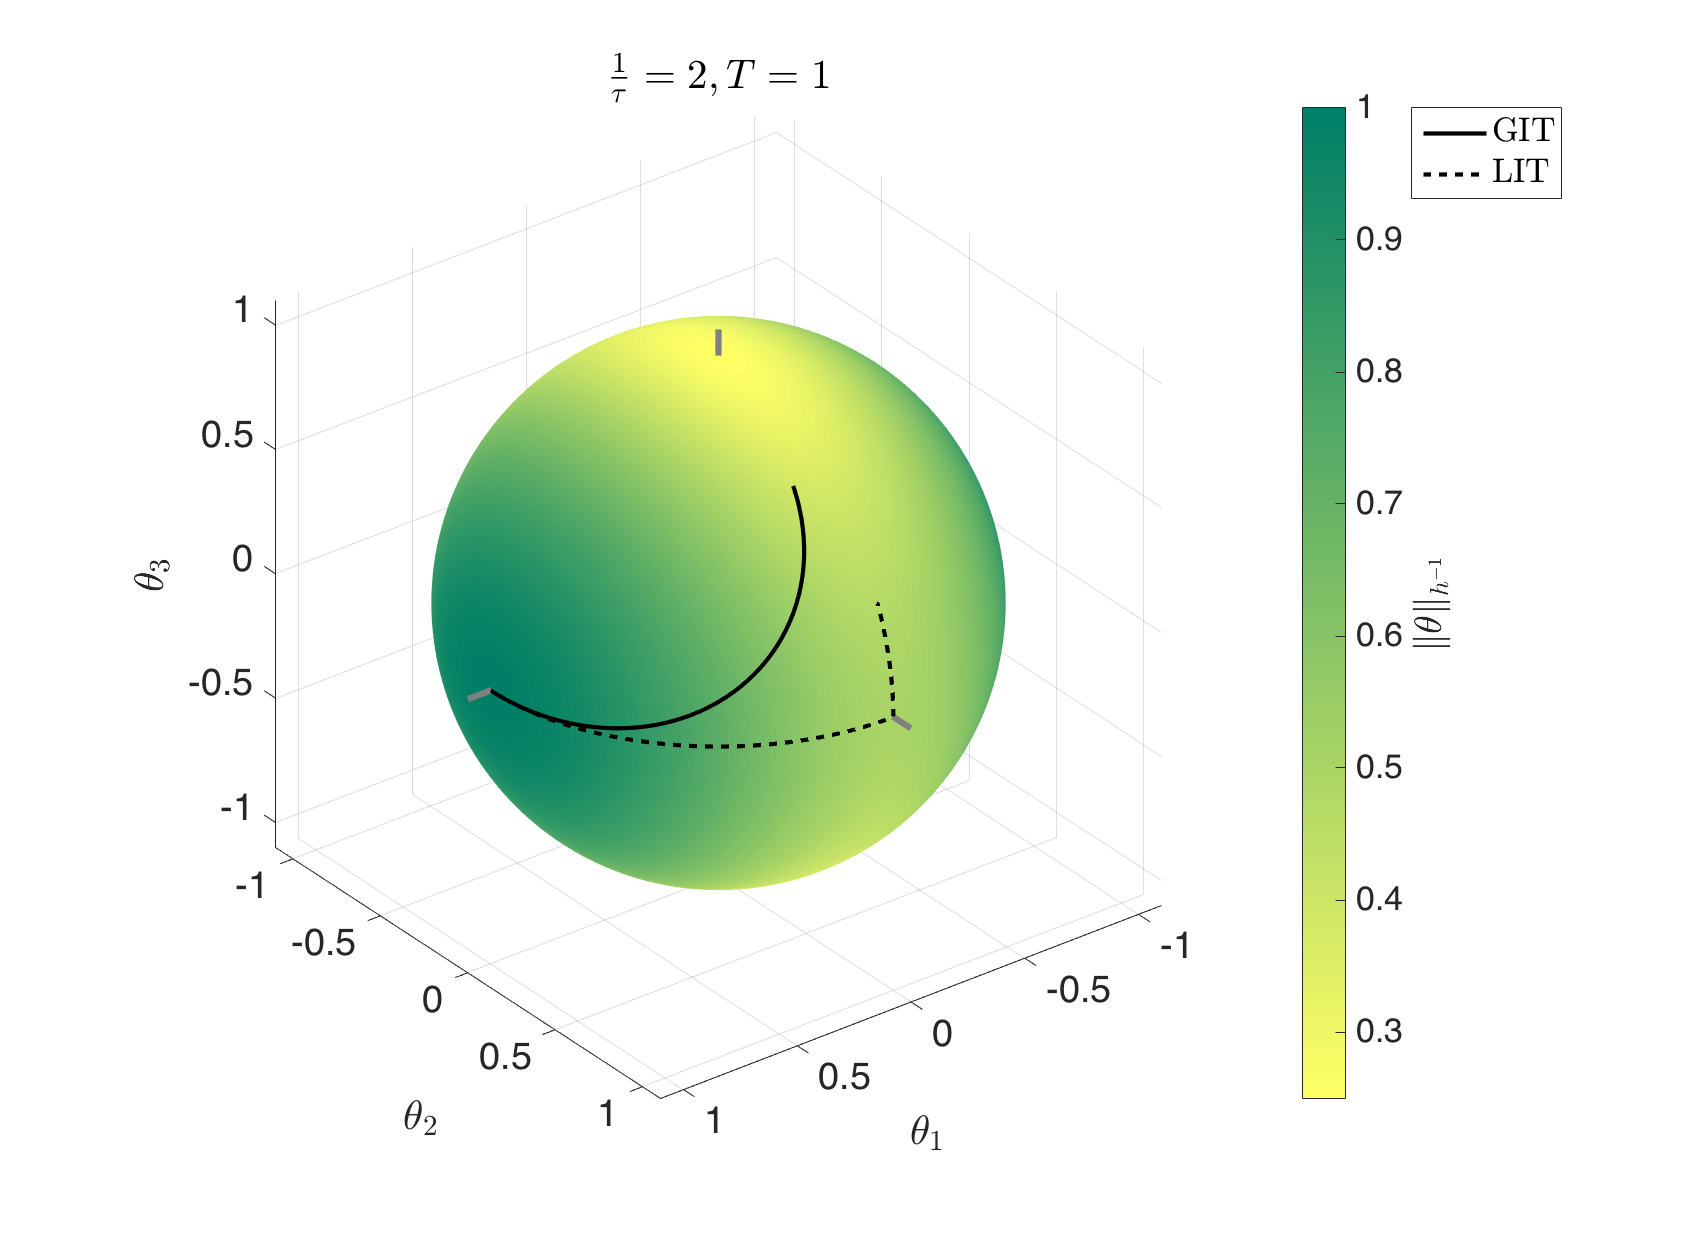
\includegraphics[width=0.7\textwidth]{ch-shellmodel/images/trajectories}
	\caption{Global-in-time and local-in-time trajectories for 3-shell model with $\frac{1}{\tau}=2$ and $T=1$ confined to a sphere with a radius given by the conserved quantity $\|\theta\|_{l^{2}}$. The color indicates the degree of mixing quantified by the mix-norm $\|\theta\|_{h^{-1}}$. }
	\label{fig:trajectories}
\end{figure*}

Using parameters $1/\tau = 2$ and $T=1$, we numerically computed $\omega \approx 1.249$ from (\ref{eq:nonlinear_system}). Thus, (\ref{eq:3_shell_optimal_control}) and (\ref{eq:3_shell_state_solution}) are known functions of time. With these parameters, the local-in-time and global-in-time trajectories evolve on a sphere with a radius defined by $\|\theta(0)\|_{l^{2}}$ in $\theta$-state space. And, the global-in-time strategy `takes a shortcut' past the $\theta_{2}$ axis relative to the local-in-time strategy as shown in figure \ref{fig:trajectories}. This short-cutting feature generalizes to truncated shell models with larger $N$ as shown in the next section.

When $ \frac{1}{\tau} =\frac{1}{\tau^{*}}\equiv\frac{\sqrt{3}\pi }{2T} $, the optimal control is given by
\begin{equation}
	\label{eq:proposed_control}
	k_{1}u_{1}=\frac{1}{\tau^{*}}\cos(\omega^{*} t) \quad
	k_{2}u_{2}=\frac{1}{\tau^{*}}\sin(\omega^{*} t).
\end{equation}
where  $\omega^{*}=\frac{\pi}{2T}$. (\ref{eq:proposed_control}) satisfies the budget constraint. This form is again the same as (\ref{eq:3_shell_optimal_control}) and therefore the state vector solution is given by (\ref{eq:3_shell_state_solution}) with $\frac{1}{\tau}=\frac{1}{\tau^{*}}$ and $\omega =\omega^{*}$. By evaluating (\ref{eq:3_shell_state_solution}) at $t=T$, we find that $\theta(T) = (0, 0, 1)^{T}$ which is the most mixed state. Therefore the proposed control (\ref{eq:proposed_control}) is a {\it global } optimum. The parameter regime with $\frac{1}{\tau}> \frac{1}{\tau^{*}}$ is not of interest since this corresponds to having excess budget. To handle this situation, introduce an inequality rather than equality in our budget constraint. If this change is made, (\ref{eq:proposed_control}) would be the optimal solution for all values $\frac{1}{\tau}> \frac{1}{\tau^{*}}$.

\subsection{Global-in-time strategy for N-shell truncated models}
\label{sec:ND_GIT_Nshell}
\begin{figure*}[!ht]
	\centering
	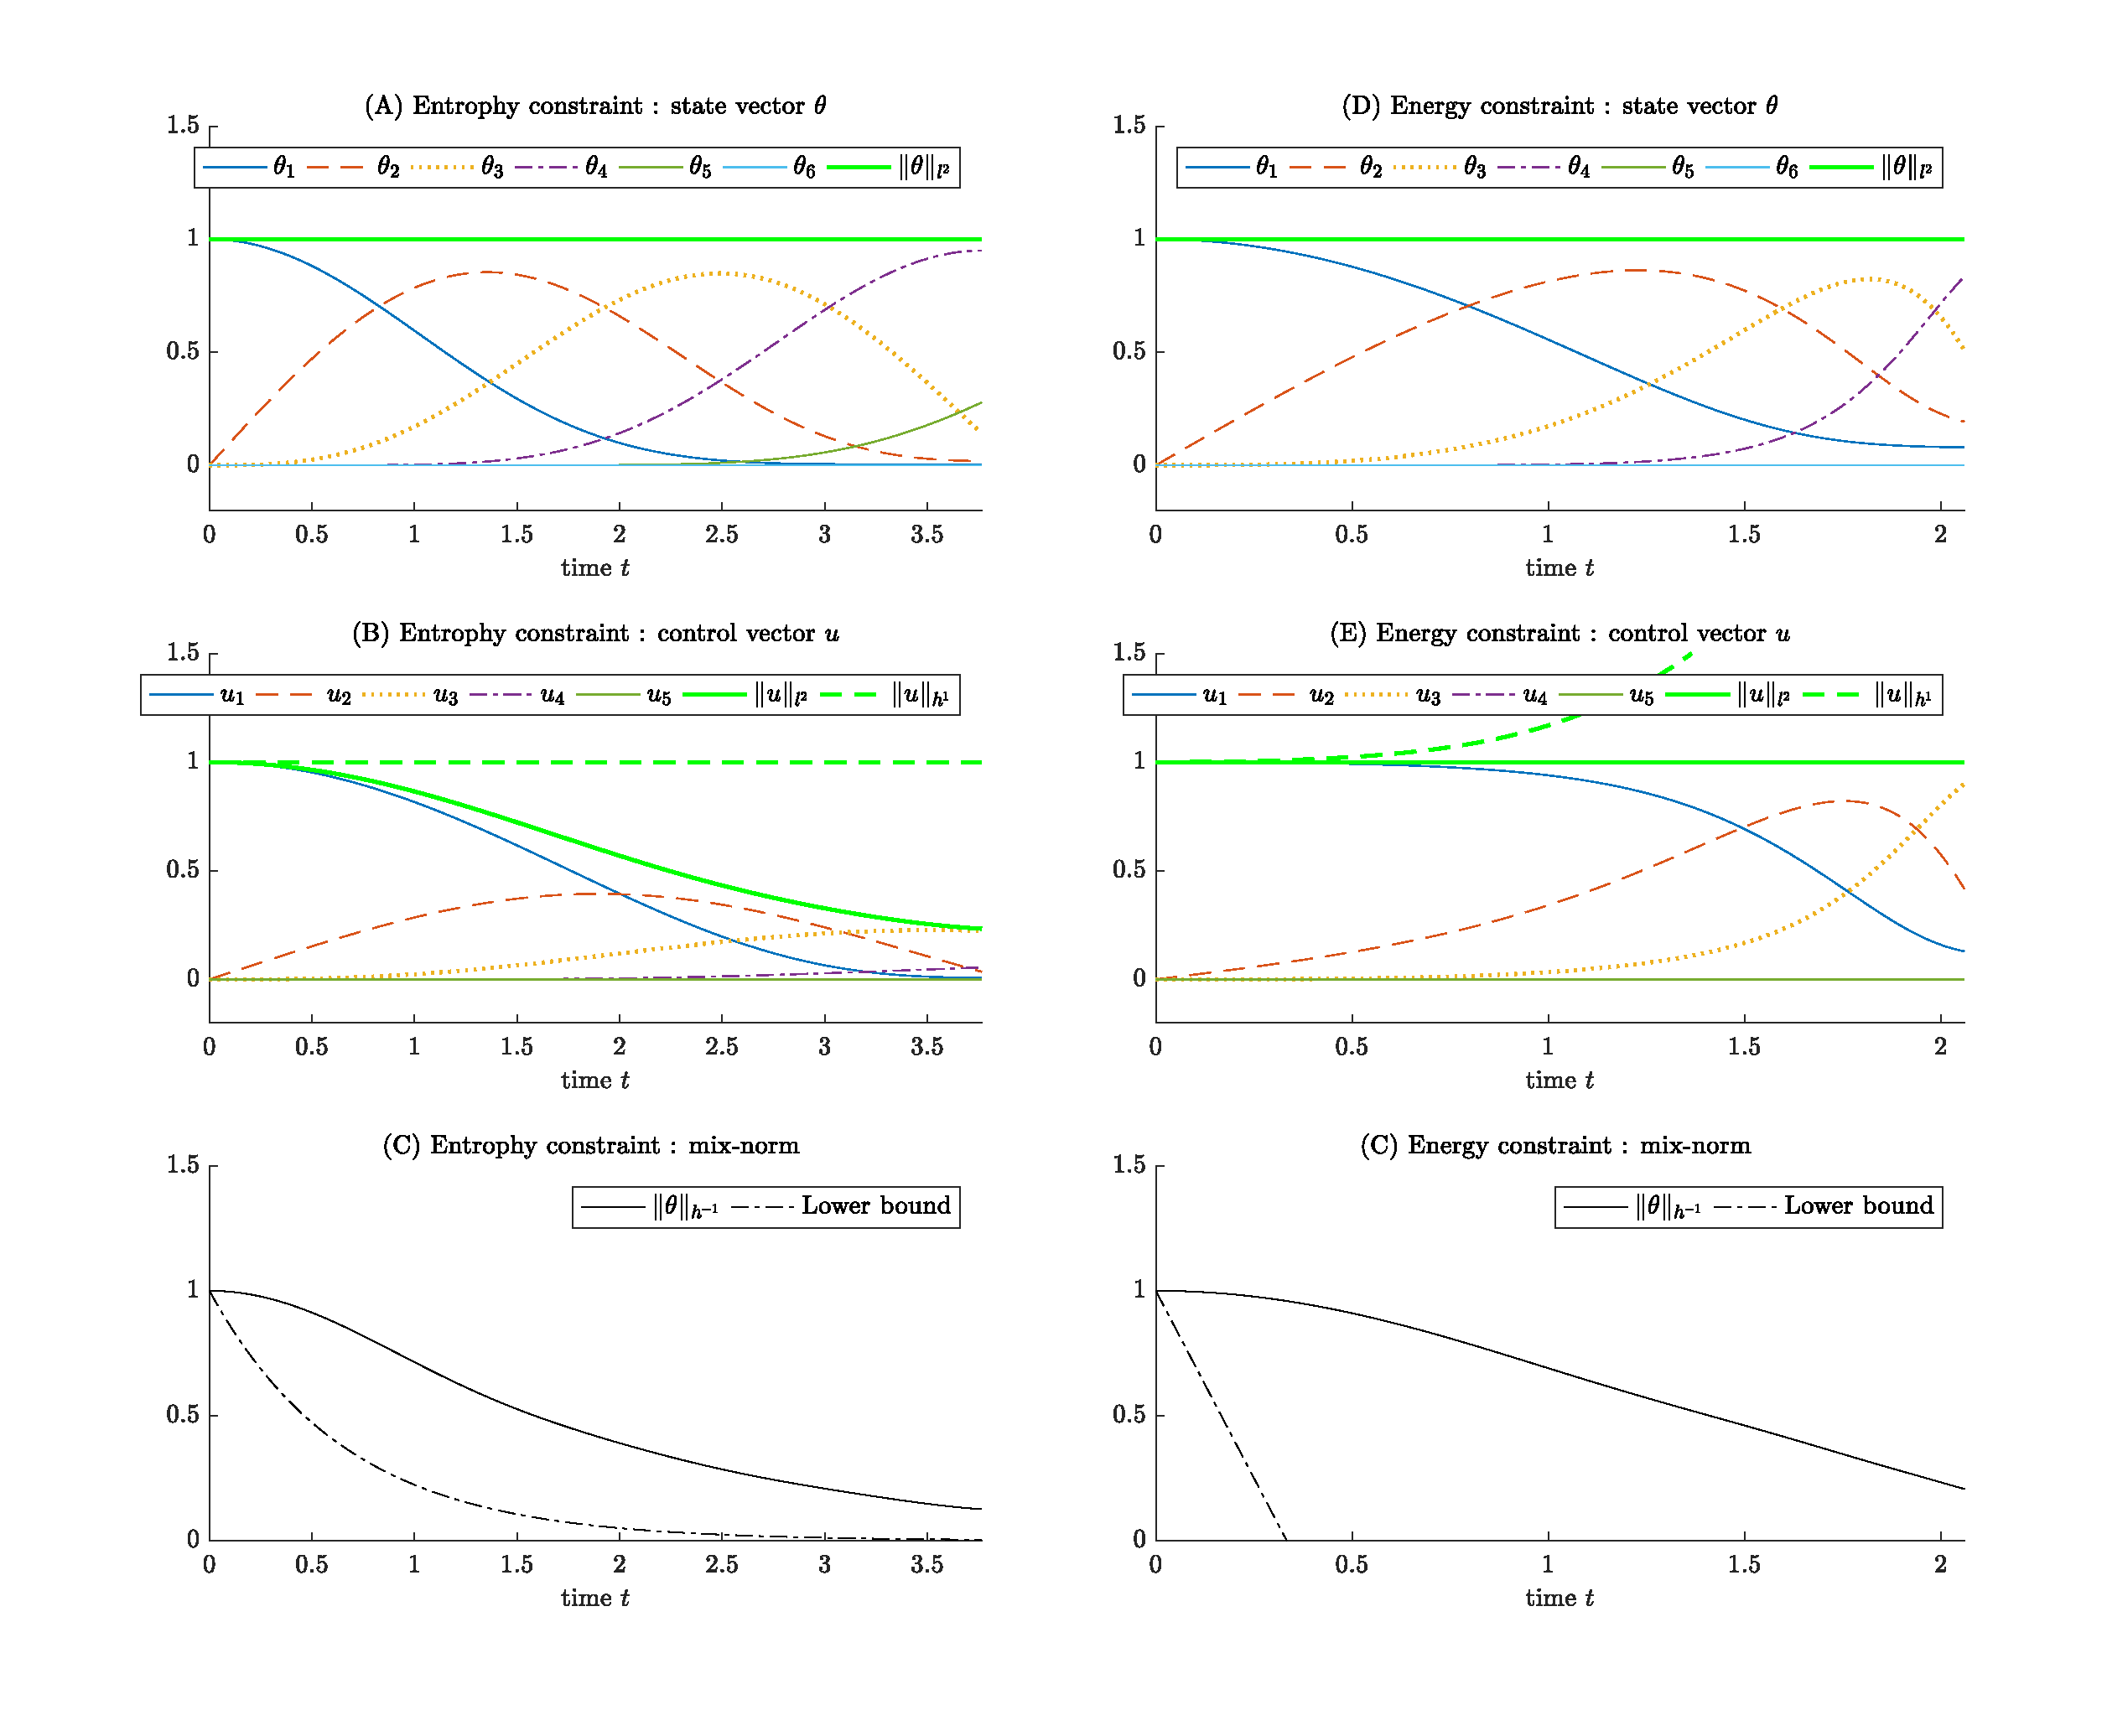
\includegraphics[width=1.0\textwidth]{ch-shellmodel/images/git_muic}
	\caption{Global-in-time strategy applied to the 6-shell truncated model starting initially from the most unmixed state. The entrophy-constrained case ($\frac{1}{\tau}=1, T=3.77 $) is shown on the left subplots where (A) shows the state, (B) shows the control, and (C) shows the mix-norm. The energy-constrained case ($U=1, T= 2.06$) is shown on the right subplots where (D) shows the state, (E) shows the control, and (F) shows the mix-norm.  }
	\label{fig:git_muic}
\end{figure*}



It is uncertain if an analytic solution can be found for arbitrary shell truncation number $N$ and constraint type (enstrophy or energy). However, it is possible to solve the general case numerically by using a gradient-based method (classical gradient descent adapted to converge to a saddle point rather than a minimum).  The algorithm begins with an initial guess for $u(t)=u^{(0)}(t)$ and $\mu=\mu^{(0)}$. Given $u$, we numerically integrate (\ref{eq:first_variation_state}) forward in time to determine $\theta(t)$. We then use the terminal condition $\phi_{n}(T)=\frac{\theta_{n}(T)}{k_{n}^2}$ to provide an `initial' condition for $\phi$ when evolving (\ref{eq:first_variation_adjoint}) backwards in time. We relax the optimality condition (\ref{eq:first_variation_optimality}) and budget constraint (\ref{eq:first_variation_constraint}). Our update rules for $u^{(k)}$ and $\mu^{(k)}$ are given by


\begin{eqnarray}
	\label{eq:update_scheme}
	u^{(k+1)}_{n}&=&u^{(k)}_{n}-\nu_{u} \frac{\delta \mathcal{L}}{\delta u_{n}} \\
	\mu^{(k+1)}&=&\mu^{(k)}+\nu_{\mu} \frac{\delta \mathcal{L}}{\delta \mu_{n}}
\end{eqnarray}
where
\begin{eqnarray}
	\frac{\delta \mathcal{L}}{\delta u_{n}}&=& k_{n}\phi_{n+1}\theta_{n} - k_{n}\phi_{n}\theta_{n+1}+\mu k_{n}^{2\alpha}u_{n} \\
	\frac{\delta \mathcal{L}}{\delta \mu}&=& \frac{1}{T}\int_{0}^{T}\|u\|_{h^{\alpha}} dt - [W^{(\alpha)}]^{2}.
\end{eqnarray}
Our convergence criteria is given by
\[
	\left \| \frac{\delta \mathcal{L}}{\delta u_{n}}\right\|_{l^{\infty}}<\delta  \text{ and }
	\left|\frac{\delta \mathcal{L}}{\delta \mu}\right|<\delta
\]
where both inequalities above must be true to deem convergence with tolerance $\delta$.

Using this method, we computed the optimal solution for the 6-shell truncated model. We choose $\frac{1}{\tau} = 1$ for the enstrophy-constrained case and $U=1$ for the energy-constrained case.  Both cases are shown in figure \ref{fig:git_muic} -- this should be compared with the local-in-time strategy for both constraint types. The rate of mixing with the global-in-time strategy shows improvement over local-in-time strategy in both the enstrophy and energy constrained cases. As first seen in 3-shell truncated model, we again see the `short-cutting' feature where the state vector never visits a $\theta_{n}$ axis as seen in the local-in-time case. Although we only show the case for  $N =6$ as an example, this feature was observed for larger values of $N$. Figure \ref{fig:git_muic} also shows how the mix-norm over time compares to the lower bounds derived in Appendices \ref{appendix:lower_bound_enstorphy_nodiff} and \ref{appendix:bound_energy_no_diff}.



\section{Mixing with diffusion}
\label{sec:diffusivecase}

In this section, we will see how diffusion affects the dynamics. One key characteristic is that the quantity $\|\theta\|_{l^{2}}$ is no longer conserved as shown clearly by the relation (\ref{eq:shell_L2decay}) with positive $\kappa$.

\begin{figure*}[!ht]
	\centering
	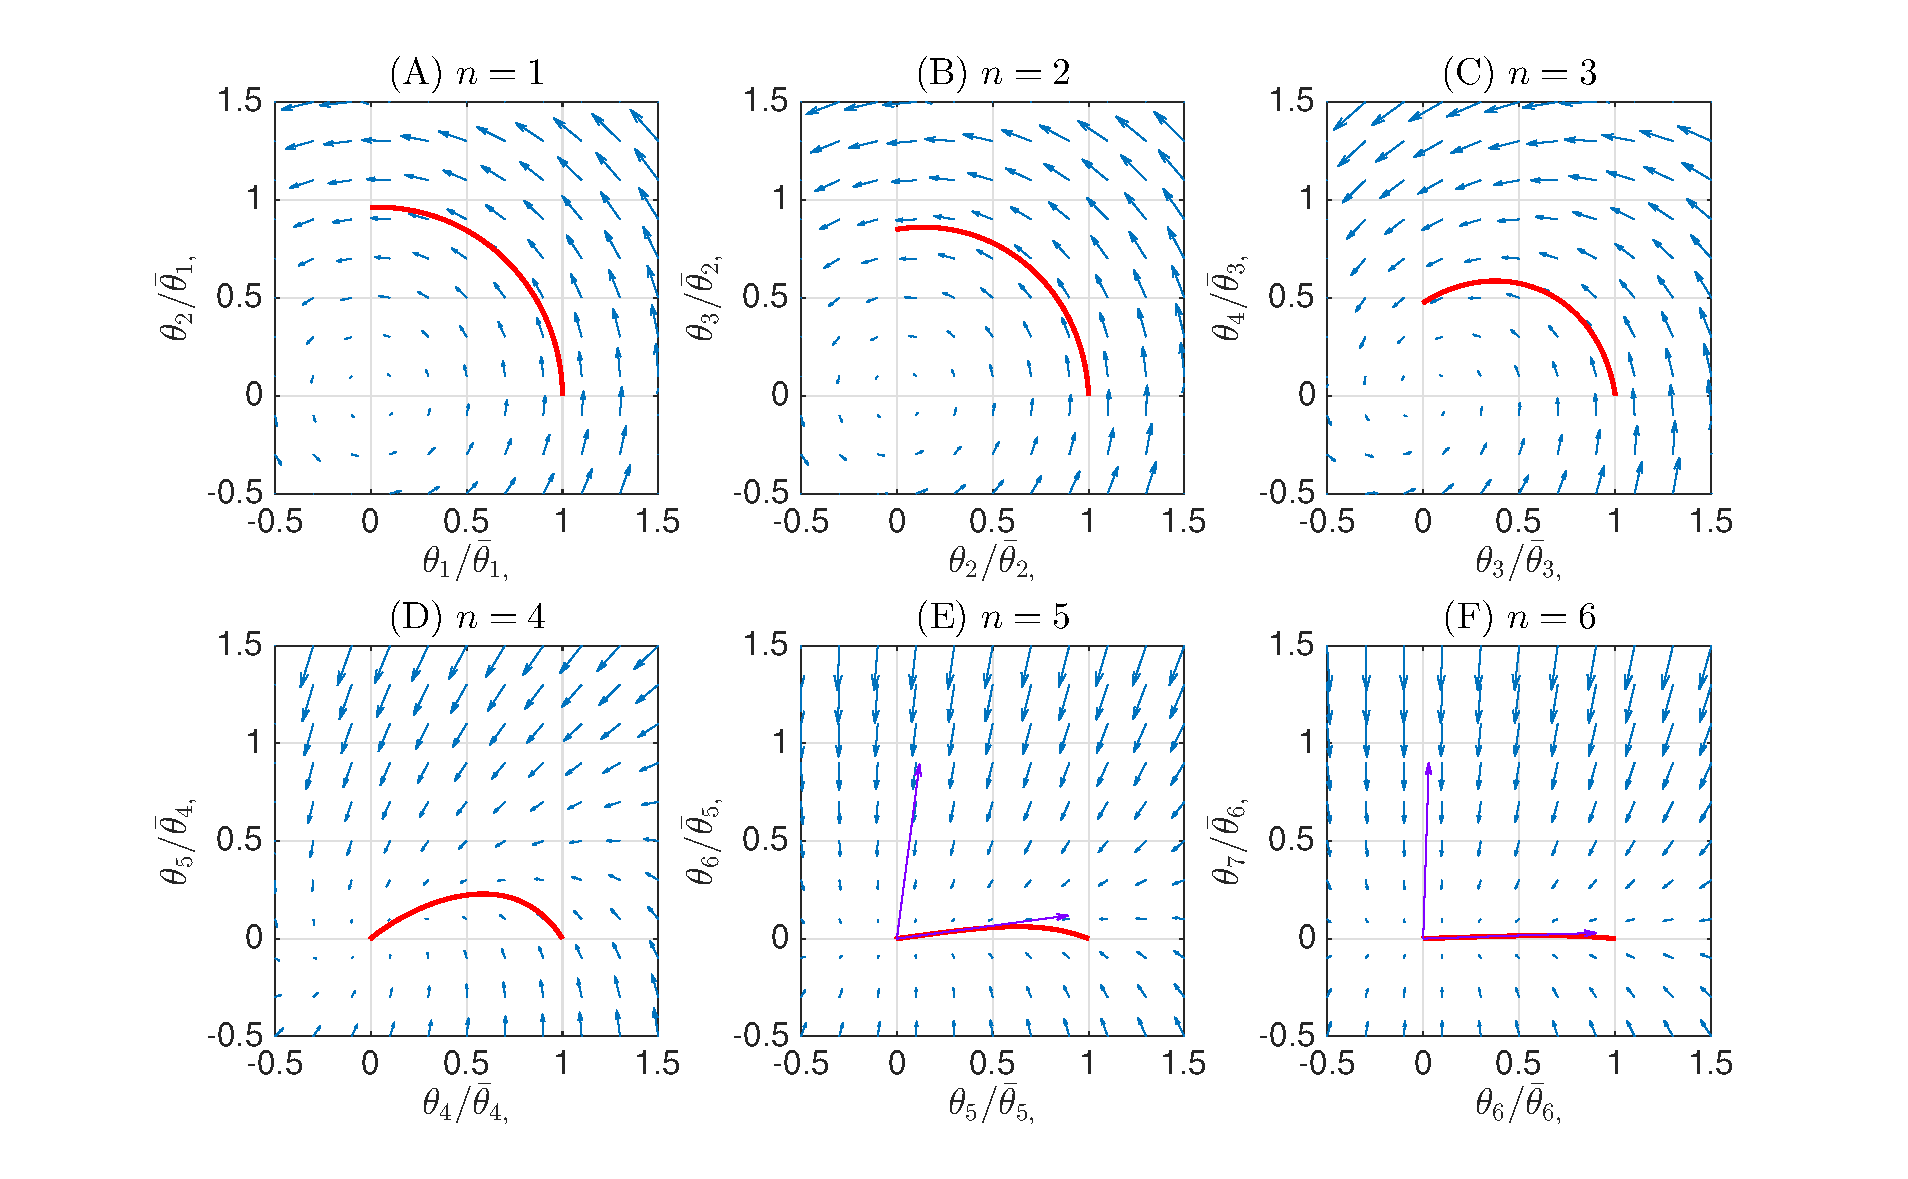
\includegraphics[width=0.8\textwidth]{ch-shellmodel/images/phase_portraits}
	\caption{Local-in-time optimal strategy with diffusion ($\kappa=0.01$) and fixed enstrophy ($1/\tau=1$). The state trajectory is indicated in red and the normalized eigenvectors are purple. The fixed point at the origin is a stable spiral for low values of $n$ and becomes a stable node when $n$ is greater than $4$.  }
	\label{fig:diffusion_phase_portraits}
\end{figure*}



\begin{figure*}[!ht]
	\centering
	\includegraphics[width=1.0\textwidth]{ch-shellmodel/images/lit_diff_muic}
	\caption{Local-in-time strategy with diffusion ($\kappa=0.01$) starting initially from the most unmixed state. The entrophy-constrained case ($\frac{1}{\tau}=1$) is shown on the left subplots where (A) shows the state, (B) shows the control, and (C) shows the mix-norm. The energy-constrained case ($U=1$) is shown on the right subplots where (D) shows the state, (E) shows the control, and (F) shows the mix-norm. Lower bounds from applying {\it Theorem 2} in Appendix \ref{appendix:pmift_impossible} are also shown in subplots (C) and (F).}
	\label{fig:lit_diff_muic}
\end{figure*}

We again consider the same initial condition and local-in-time optimization problem seen in \ref{sec:LIT_MUIC}. Recall that the initial state is the most umixed state, $\theta(0)=(1, 0, 0, \dots )^{T}$. We deal with the generalized constraint (\ref{eq:shellNN_lit_contstraint}) parameterized by $\alpha$. By employing results from the section \ref{sec:LIT}, the optimal strategy is to initially use $u_{1}=W^{(\alpha)}/k_{1}^{\alpha}$ with the other components of $u$ set to zero. Thus,  the motion will initially be in the $\theta_{1}$-$\theta_{2}$ plane with the following reduced state equation

\[
	\frac{d}{dt}\left( \begin{array}{c}
	\theta_{1} \\
	\theta_{2}\end{array} \right)
	=
	\left( \begin{array}{cc}
	-\kappa k_{1}^2 & -k_{1}u_{1} \\
	k_{1}u_{1} & -\kappa k_{2}^2  \end{array} \right)
	\left( \begin{array}{c}
	\theta_{1} \\
	\theta_{2}\end{array} \right).
\]
Once the state encounters the axis $(0,1,0,0, \dots)^{T}$, the optimal strategy will switch to $u_{2}= W^{(\alpha)}/k_{2}^{\alpha}$ until the state encounters the next axis $(0,0,1,0,0 \dots)^{T}$. This trend will continue as long as the state keeps visiting each axis. In general, the motion is governed piecewise in time by the following state equation
\begin{equation}
	\frac{d}{dt}\left( \begin{array}{c}
	\theta_{n} \\
	\theta_{n+1}\end{array} \right)
	=
	\left( \begin{array}{cc}
	-\kappa k_{n}^2 & -k_{n}u_{n} \\
	k_{n}u_{n} & -\kappa k_{n+1}^2  \end{array} \right)
	\left( \begin{array}{c}
	\theta_{n} \\
	\theta_{n+1}\end{array} \right)
\end{equation}
after visiting the $n$th axis where $u_{n}=W^{(\alpha)}/k_{n}^{\alpha}$. The eigenvalue problem can be solved to produce the eigenvalues,

\begin{equation}
\label{eq:eigenvalues_lit}
	\lambda_{\pm}=-\frac{1}{2} \kappa(k_{n+1}^2 + k_n^2) \pm \frac{1}{2}\beta_{n}^{(\alpha)}
\end{equation}
where $\beta_{n}^{(\alpha)}=\sqrt{\kappa^{2}(k_{n+1}^2 - k_n^2)^2 - 4 k_n^{2(1-\alpha)} [W^{(\alpha)}]^2 }$, and eigenvectors, in the $\theta_{n}$-$\theta_{n+1}$ plane,

\begin{equation}
	\Theta_{\pm} = \left(
	\begin{array}{c}
		\frac{1}{2} \kappa(k_{n+1}^2 - k_n^2) \pm \frac{1}{2} \beta_{n}^{(\alpha)}\\
		k_n^{1-\alpha}W^{(\alpha)}
	\end{array}
	\right).
\end{equation}
Define $\Theta_n (t)= (\theta_n(t) , \theta_{n+1}(t) )^{T}$. With the initial condition $\Theta_n (0) = (\bar{\theta}_{n}, 0)$ where $\bar{\theta}_{n}$ is the initial value of $\theta_{n}$ at the $n$th time interval, we obtain the solution
\begin{equation}
	\Theta_{n}(t)= \frac{\bar{\theta}_{n}}{\beta_{n}^{(\alpha)}} \left[e^{\lambda_{+}t}\Theta_{+}- e^{\lambda_{-}t}\Theta_{-} \right].
\end{equation}

The fixed point at the origin is a stable spiral for low values of $n$. However, when
\begin{equation}
\label{eq:critical_n}
	n > n_{c} = \frac{1}{1+\alpha}\log_{2}\left(\frac{2 W^{(\alpha)}}{3 \kappa k _{0}^{1+\alpha}}\right),
\end{equation}
the origin transitions to a stable node. At this point, the trajectory {\it cannot } move to the next plane since it must intercept the $\theta_{n+1}$ axis to do so. Figure \ref{fig:diffusion_phase_portraits} shows how the phase portrait changes with shell number $n$ for the enstrophy-constrained case. Figure \ref{fig:lit_diff_muic} shows the local-in-time strategy for both the fixed enstrophy and energy cases. In other words, it is no longer optimal to keep progressing to the next shell.  This result demonstrates that even the slightest degree of diffusion prohibits the local-in-time strategy from performing perfect mixing in finite time which was possible with the perfectly non-diffusive case ($\kappa=0$).

After seeing how diffusion can drastically change the system behavior under the local-in-time scheme, it is natural to ask ``Is perfect mixing in finite time impossible?'' For the enstrophy-constrained case, we apply {\it Theorem 2} in Appendix \ref{appendix:pmift_impossible} to the initial condition $\theta(0)=(1, 0, 0 , \dots )^{T}$ with $\kappa=0.01$ and $\tau=1$. We find the lower bound on the mix-norm,
\begin{equation}
\hmone{\theta(t)}\geq A\exp(r_{+}t) 
\end{equation}
where $A =   0.0625$ and $r_{+}\approx -2.69249$. For the energy-constrained case with identical parameters and initial condition, we have the lower bound,
\begin{equation}
\hmone{\theta(t)}\geq A\exp(r_{+}t) 
\end{equation}
where $A =   0.007$ and $r_{+}\approx -199.805$. This shows that perfect mixing in finite time is indeed impossible with diffusion.


\begin{figure*}[!ht]
	\centering
	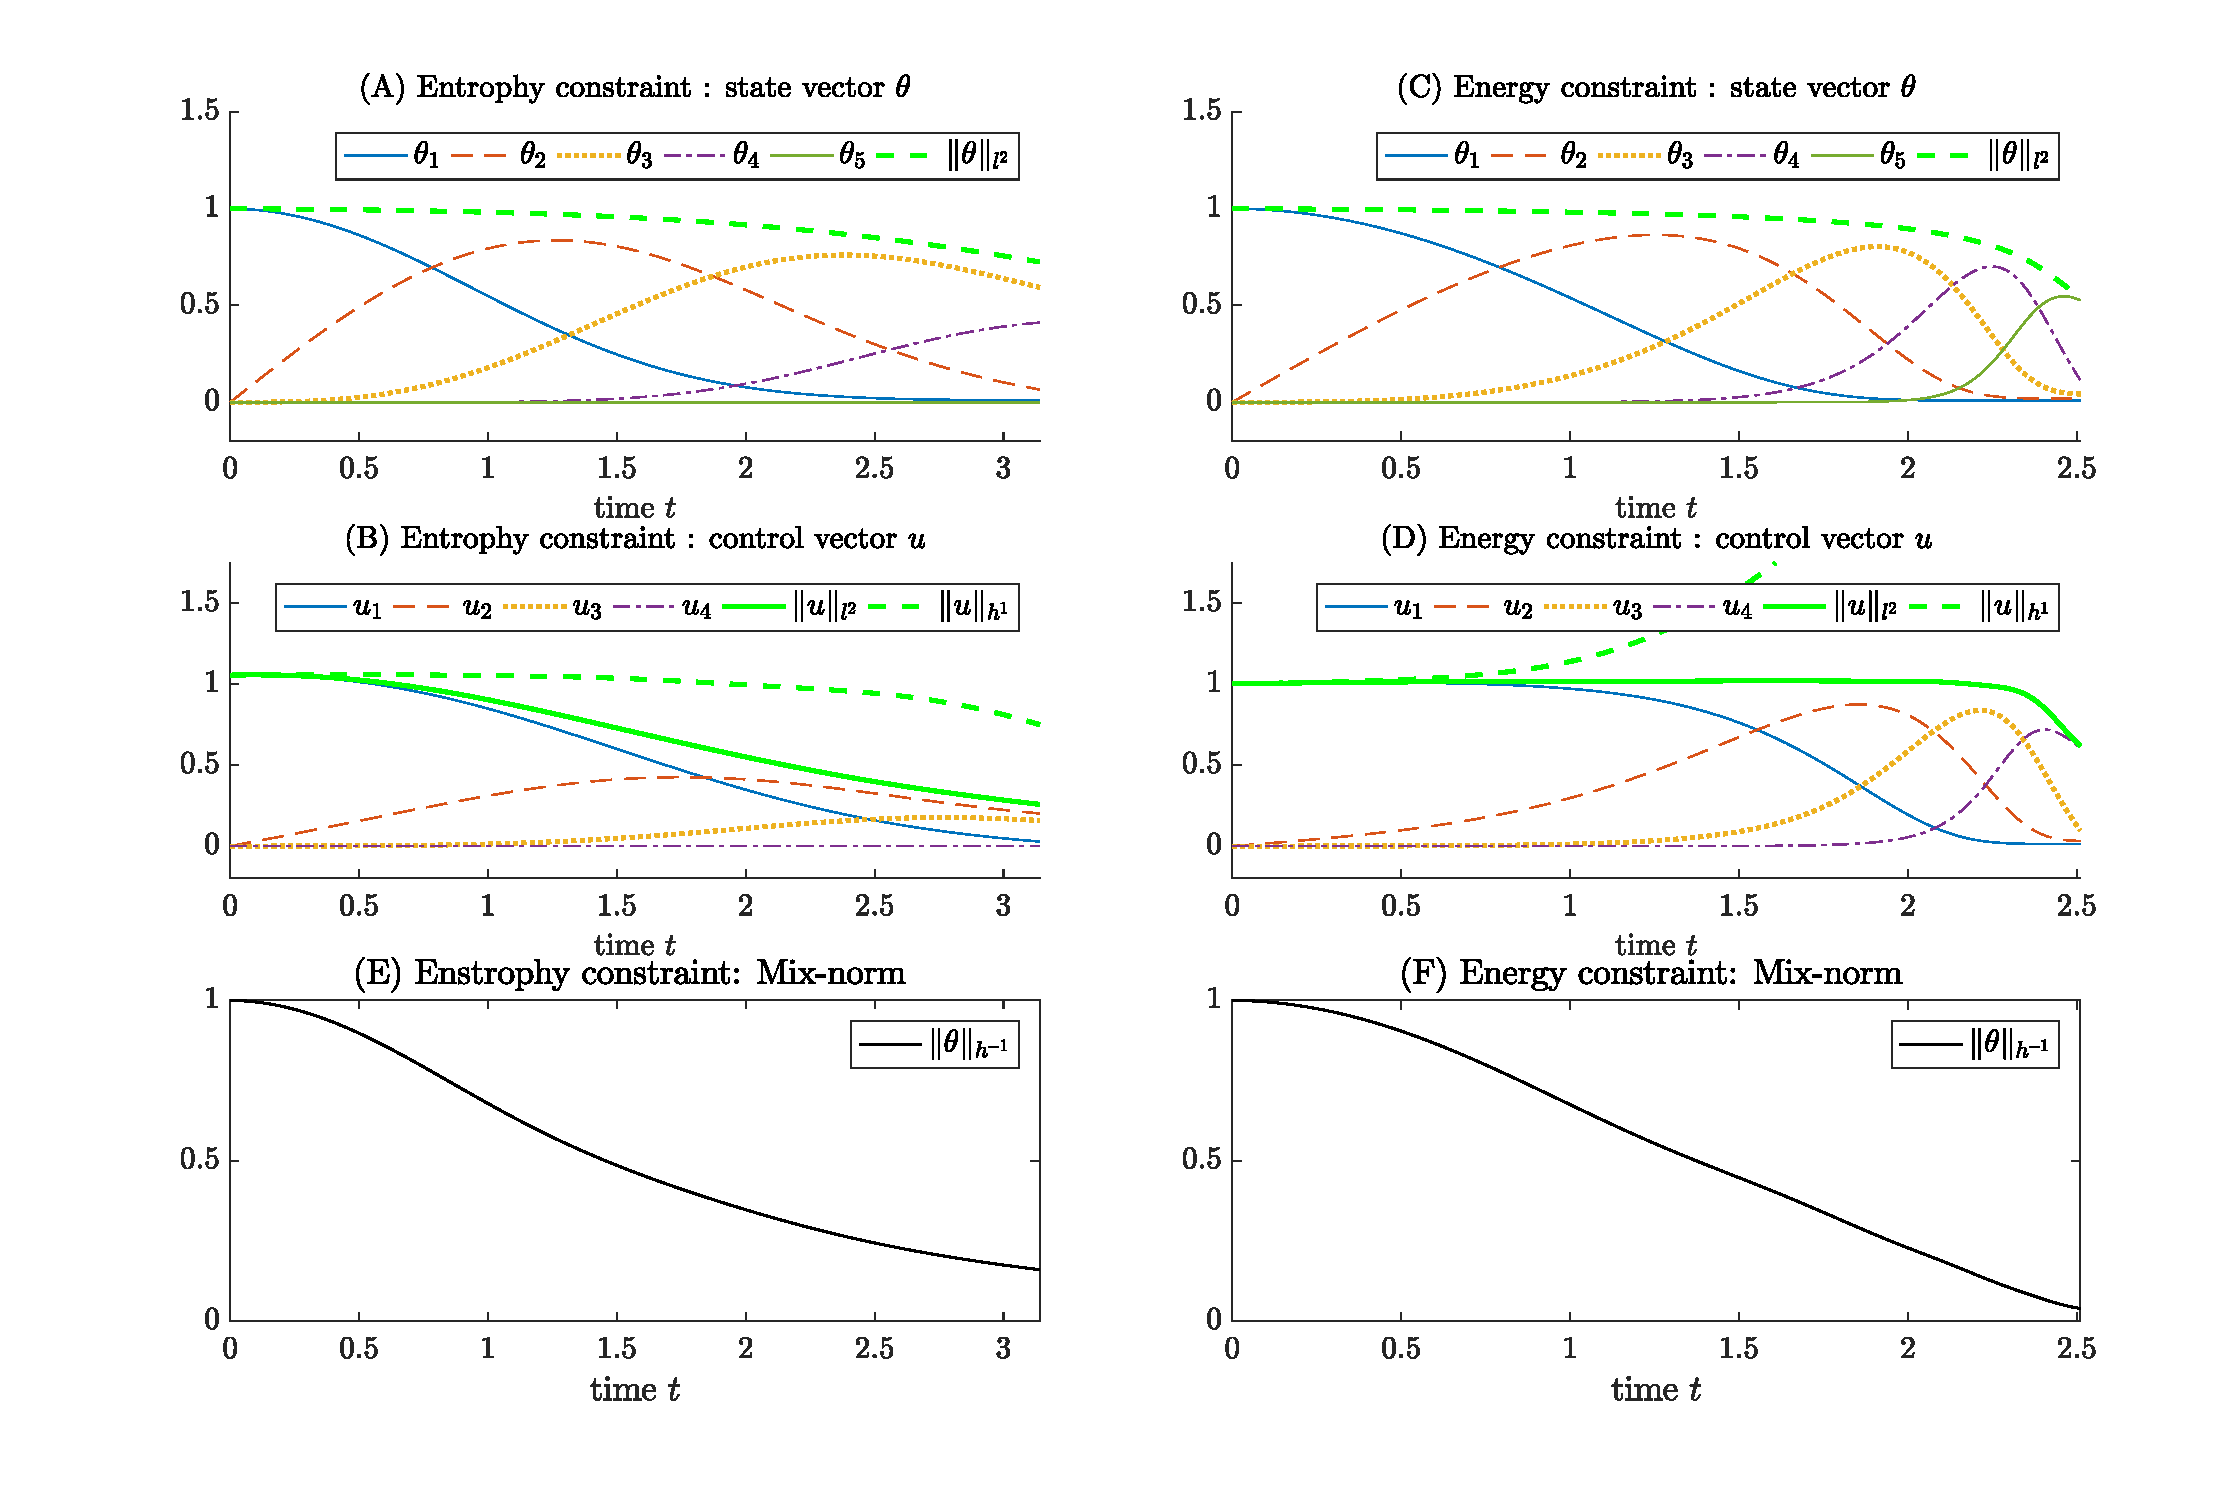
\includegraphics[width=0.9\textwidth]{ch-shellmodel/images/git_diff_muic}
	\caption{Global-in-time strategy applied to truncated shell model ($N=5$) with diffusion ($\kappa=0.01$) starting initially from the most unmixed state. The entrophy-constrained case ($\frac{1}{\tau}=1, T=\pi$) is shown on the left subplots where (A) shows the state, (B) shows the control, and (C) shows the mix-norm. The energy-constrained case ($U=1,T= 0.8\pi$) is shown on the right subplots where (D) shows the state, (E) shows the control, and (F) shows the mix-norm. }
	\label{fig:git_diff_muic}
\end{figure*}


For global-in-time optimization, we use the same numerical scheme detailed in section \ref{sec:ND_GIT_Nshell} here with $\kappa\neq 0$ in equation (\ref{eq:first_variation}). Figure \ref{fig:git_diff_muic} shows the numerical solution for a truncated shell model with $N=5$ and $\kappa=0.01$. The global-in-time strategy appears similar to that with non-diffusive situation in the sense that we see the feature of `short-cutting' relative to local-in-time strategy. We also notice the expected overall decay of the $l^{2}$ norm of $\theta$. We see that the optimal control no longer conserves energy or enstrophy with diffusion. Specifically, we see that it is optimal to use more of the budget earlier on rather than later for both the energy and enstrophy constrained cases.

\section{Discussion}
\label{sec:discussion_shell}
We first focused on mixing without diffusion. The enstrophy-constrained local-in-time strategy exhibited exponential decay while energy-constrained local-in-time strategy showed linear decay --- and hence perfect mixing in finite time. We obtained an analytic solution to the global-in-time optimization problem of the 3-shell truncated model by using methods from nuclear magnetic resonance. The global-in-time strategy applied to the 3-shell truncated model showed an improvement on the mixing rate relative to that of the local-in-time strategy by using a short-cutting method (illustrated in figure \ref{fig:trajectories}). This short-cutting feature generalized to models with higher truncation number $N$. We were surprised to find that it is optimal to use the (energy or enstrophy) budget uniformly in time (rather than consuming more budget earlier than later or vice versa). This is consistent with the work of Mathew {\it et al.} \cite{Mathew2007b} that demonstrated this feature in the partial differential equation context.

Mixing with diffusion was explored and demonstrated interesting effects.  Perfect mixing in finite time for the local-in-time strategy, while constraining either energy or enstrophy, becomes {\it impossible} (recall that it was at least possible for the energy-constrained case without diffusion). The local-in-time dynamics were restricted to $\theta_{n}$-$\theta_{n+1}$ planes piecewise in time similar to that of the local-in-time strategy seen without diffusion. As the state vector progressed to $\theta_{n}$-$\theta_{n+1}$  planes of larger $n$, the diffusive terms progressively dominate over the advective terms in our shell model. Thus, a plane is eventually reached where it is no longer advantageous to progress to the next plane. This suggests that we have succeeded at mixing to a length scale where diffusion can then take over. For energy-constrained flow, this length scale is 
\begin{equation}
\label{eq:batchelor_scale_energy}
l_{u}=\frac{3}{2}\kappa / U.
\end{equation}
For the enstrophy-constrained case, this length scale is  
\begin{equation}
\label{eq:batchelor_scale_enstrophy}
l_{\tau}=\sqrt{\frac{3}{2}\kappa \tau}
\end{equation}
which is naturally interpreted as the Batchelor length scale in turbulent mixing theory \cite{Dimotakis2005,Holzer1994b,Shraiman2000a,Batchelor1959a, Corrsin1951,Obukhov1949}. In fact, (\ref{eq:batchelor_scale_enstrophy}) has the same scaling in molecular diffusivity $\kappa$ and rate-of-strain $1/\tau$ as the turbulent theory type. Local-in-time optimization may suggest that we should mix the tracer concentration until we arrive at these small critical length scales.

But, how should one use a flow intensity budget over time during this approach to small scales? For this, we turn to global-in-time optimization.  Recall that global-in-time optimization without diffusion revealed that it is optimal to use your budget uniformly in time. We find however that this is no longer the case with diffusion. It is optimal to use more of the (energy or enstrophy) budget earlier than later. Therefore, this suggests that budget use is more effective at larger scales away from the Batchelor length scale.

These observations prompt the following questions: ``Will diffusion always dominate advection eventually?'' and ``If so, does this mean that perfect mixing in finite time is impossible?'' We showed in Appendix  \ref{appendix:pmift_impossible} that perfect mixing in finite time is indeed impossible for the enstrophy and energy local-in-time constraints by producing exponential lower bounds on the mix-norm in both cases. 


\begin{figure*}[!ht]
	\centering
	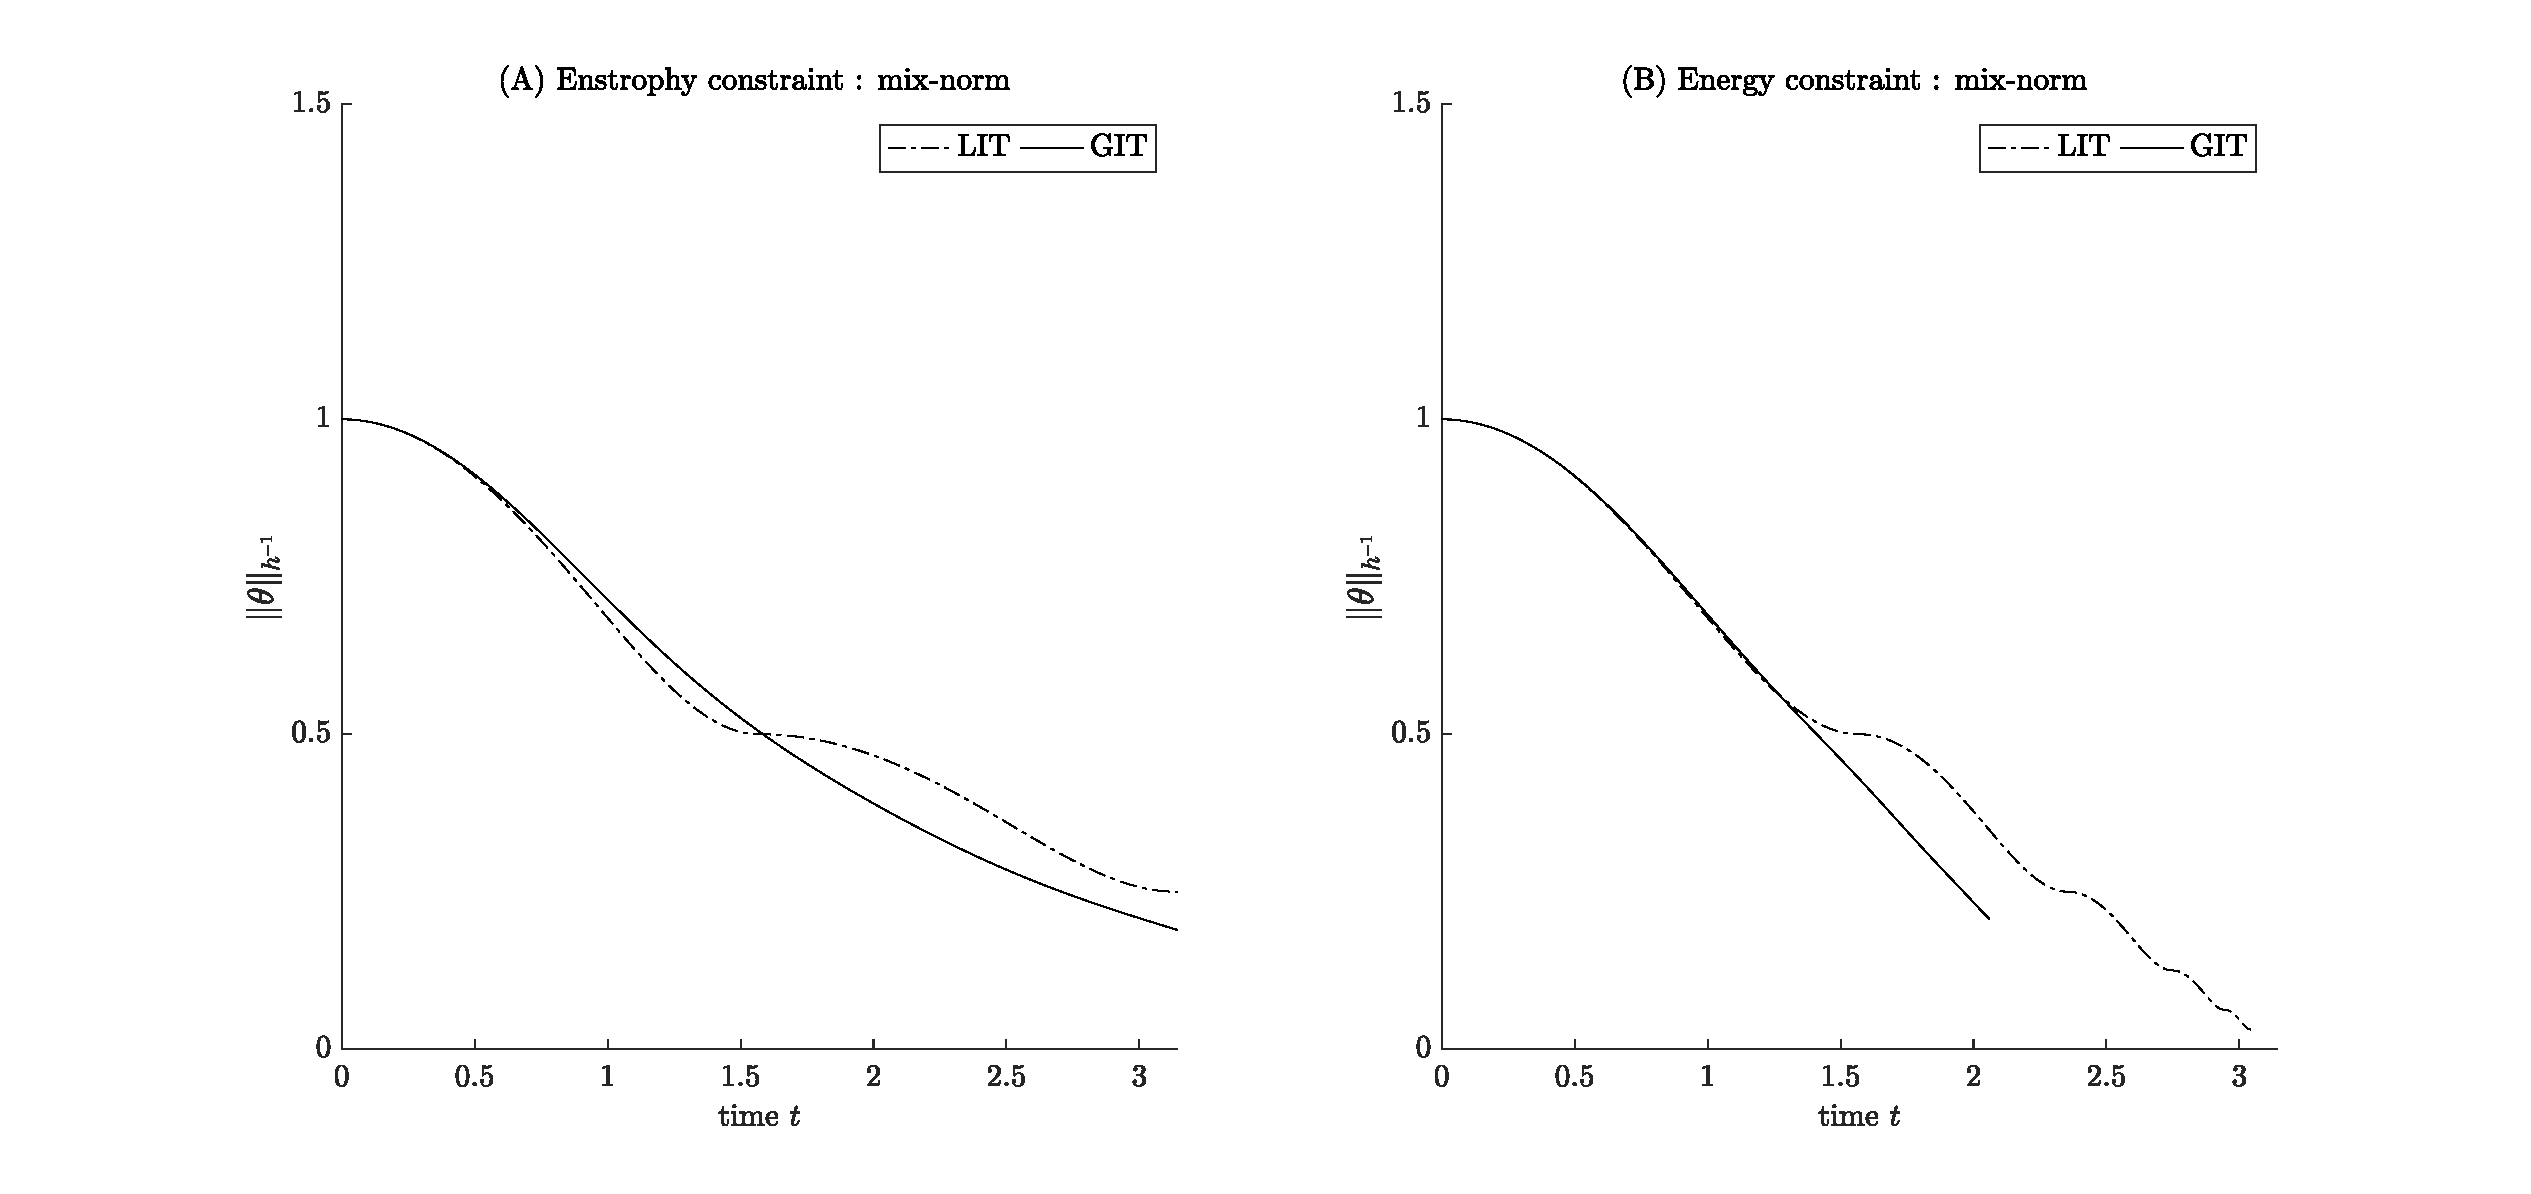
\includegraphics[width=0.8\textwidth]{ch-shellmodel/images/lit_vs_git}
	\caption{The mix-norm over time for the local-in-time (same data from figure \ref{fig:lit_muic}) and global-in-time (same data from figure \ref{fig:git_muic}) strategies applied to the 6-shell truncated shell model without diffusion. The initial condition is $\theta(0)=\mathbf{e}_{1}$. The left plot (A) shows the enstrophy-constrained case with $\tau=1$ and the right plot (B) shows the energy-constrained case with $U=1$. }
	\label{fig:lit_vs_git}
\end{figure*}
\begin{figure*}[!ht]
	\centering
	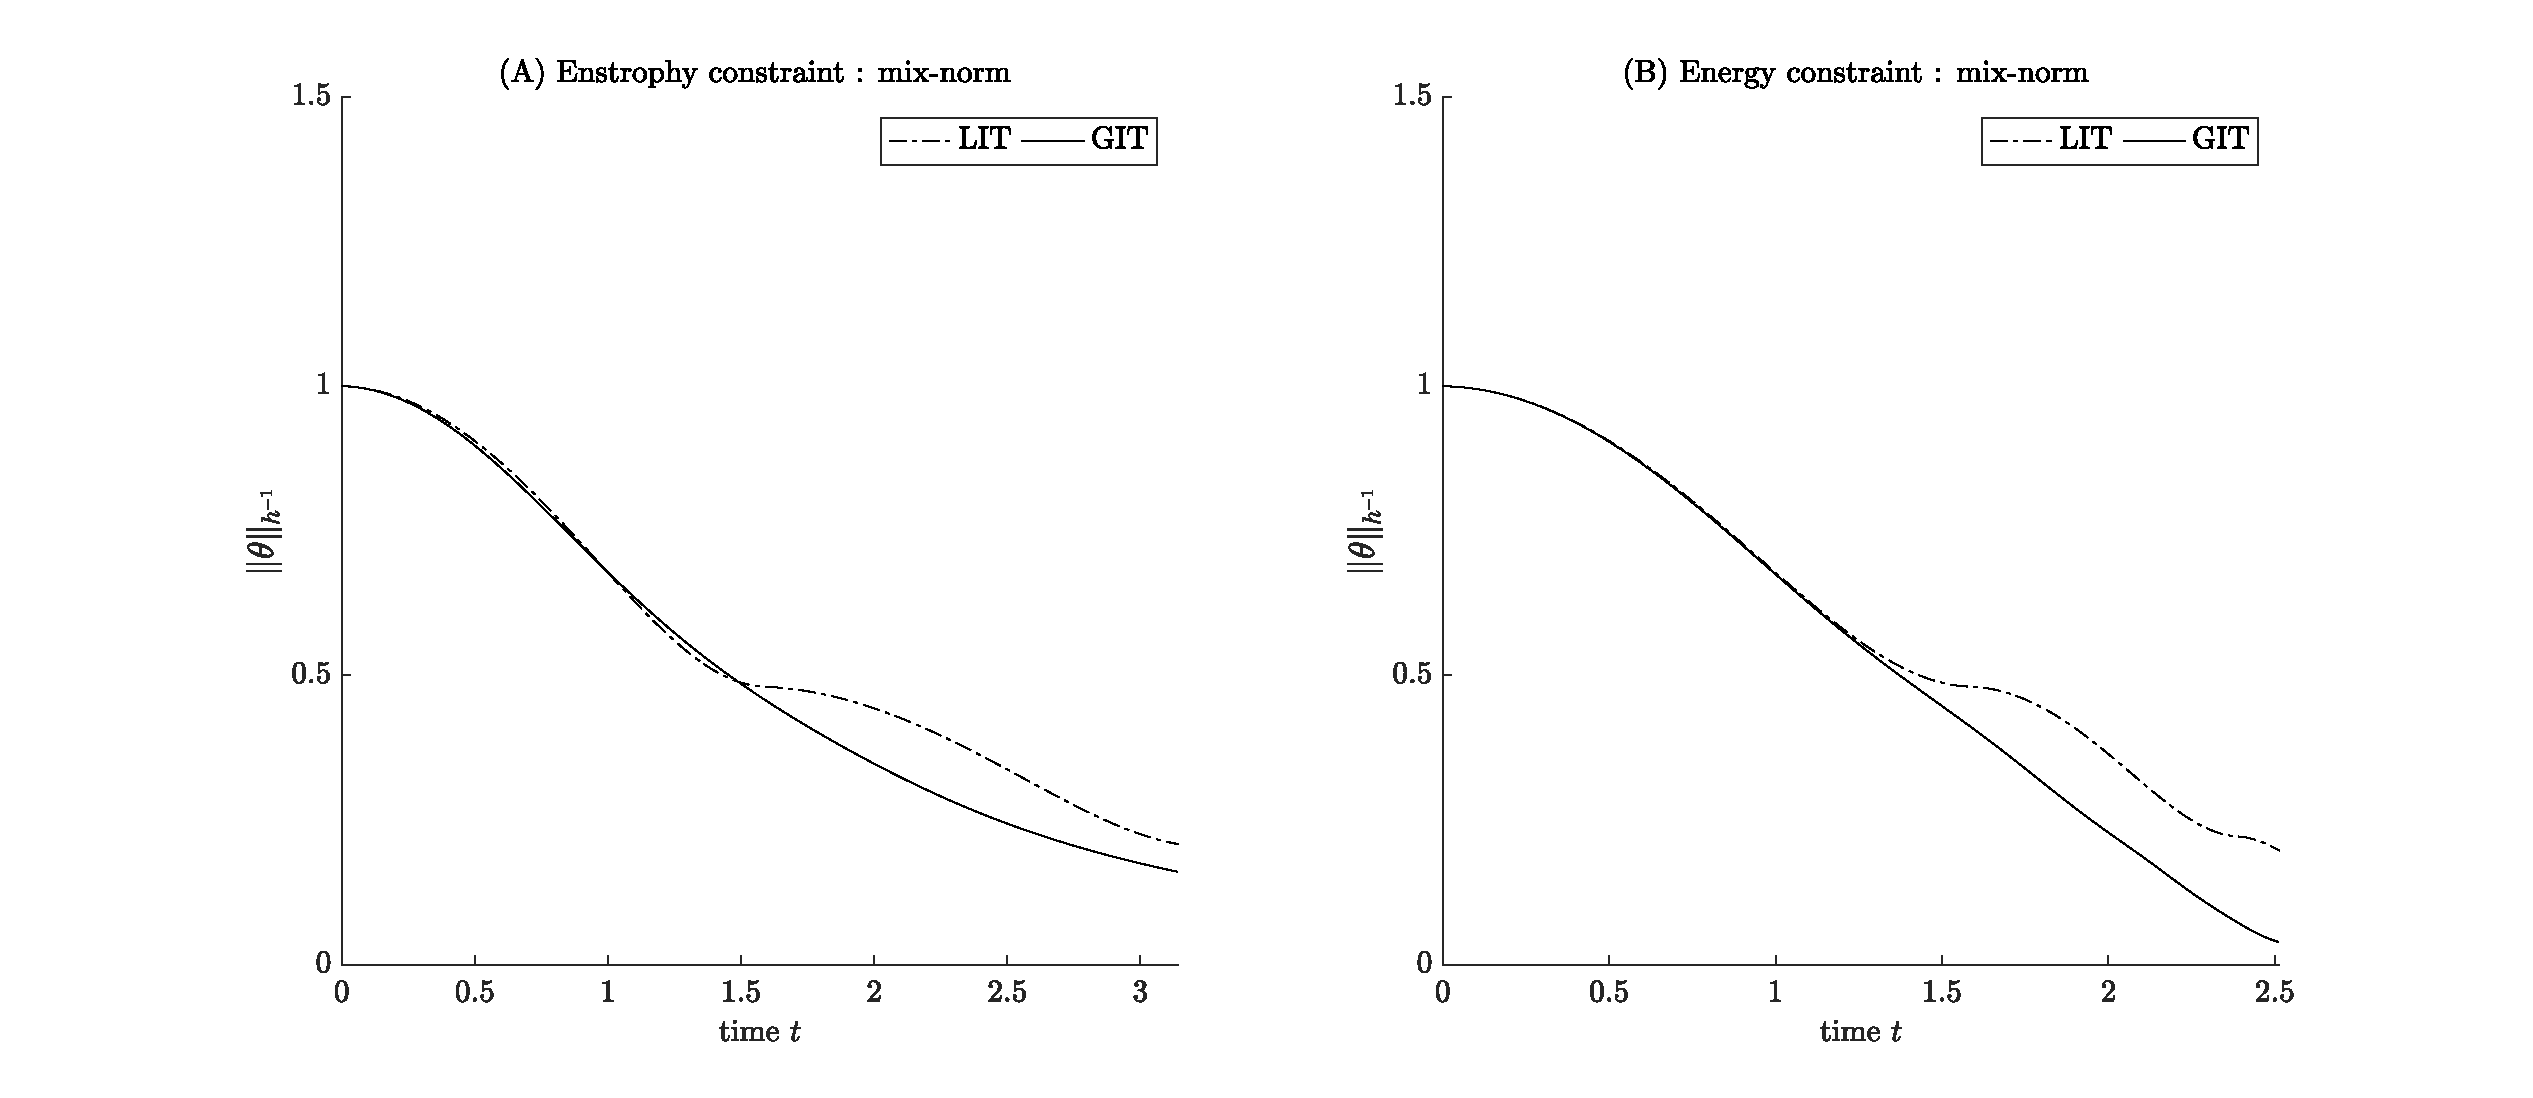
\includegraphics[width=0.9\textwidth]{ch-shellmodel/images/lit_vs_git_diff}
	\caption{The mix-norm over time for the local-in-time (same data from figure \ref{fig:lit_diff_muic}) and global-in-time (same data from figure \ref{fig:git_diff_muic}) strategies applied to the 5-shell truncated shell model with diffusion. The initial condition is $\theta(0)=\mathbf{e}_{1}$. The left plot (A) shows the enstrophy-constrained case with $\tau=1$ and the right plot (B) shows the energy-constrained case with $U=1$. }
	\label{fig:lit_vs_git_diff}
\end{figure*}

 \begin{figure*}[!ht]
	\centering
	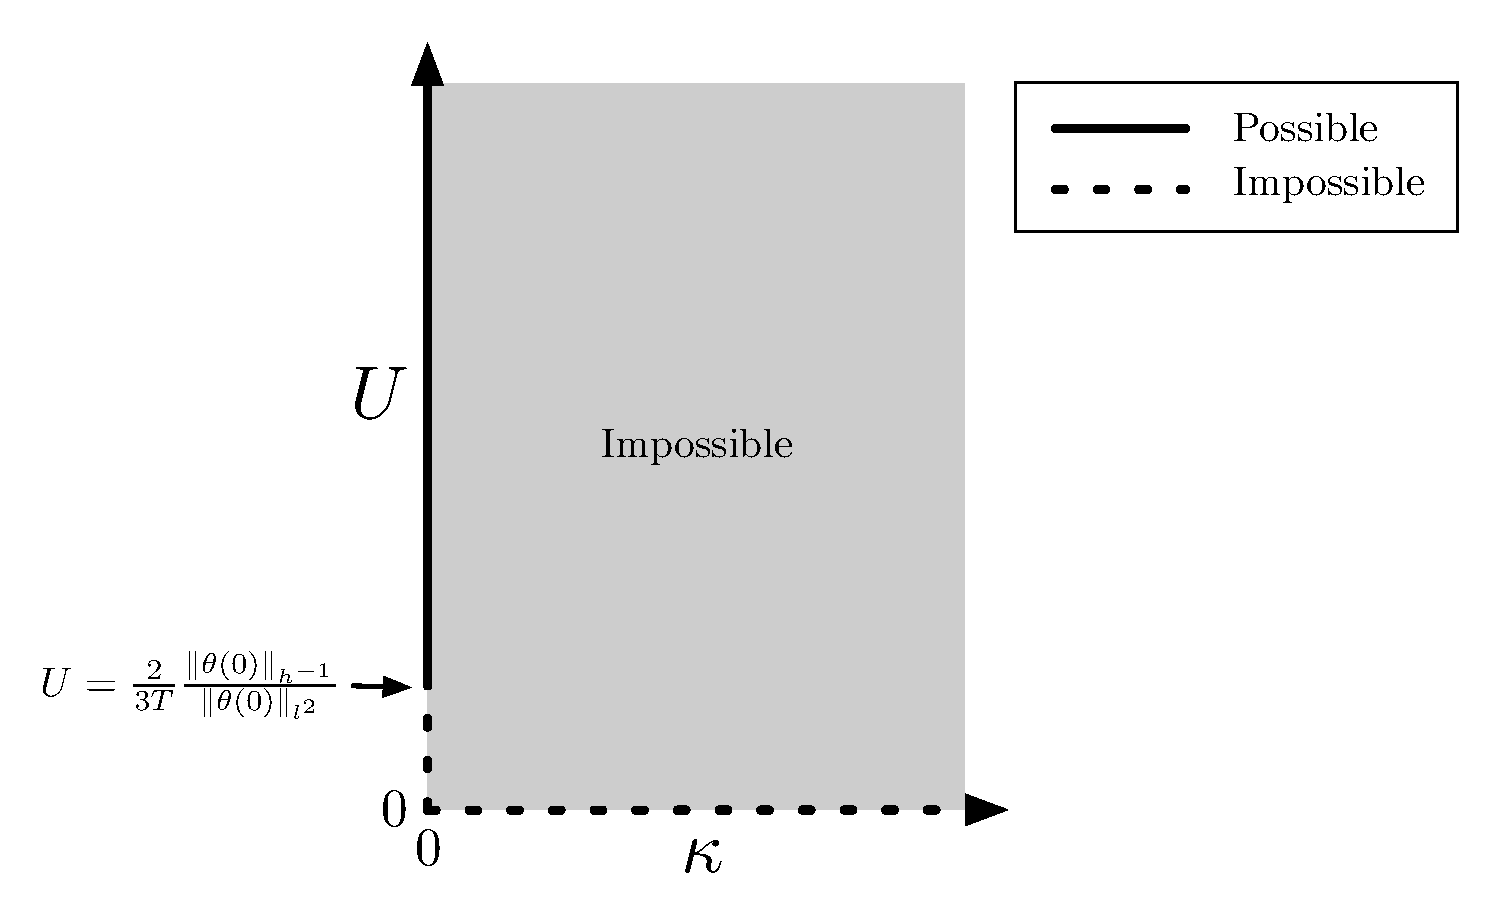
\includegraphics[width=0.5\textwidth]{ch-shellmodel/images/perfectmixing}
	\caption{The possibility of perfect mixing in finite time with energy constraint $\ltwo{u}=U$ and diffusion constant $\kappa$.}
	\label{fig:perfectmixing}
\end{figure*}


In conclusion the developed shell model preserves many known features of the partial differential equation problem. For instance, the shell model performed perfect mixing in finite time without diffusion and with an energy constraint   (Lunasin {\it et al.} \cite{JMP2012}), and showed exponential mix-norm decay without diffusion and with an enstrophy constraint  (Seis \cite{CS2013} and Iyer {\it et al.} \cite{GI2014}).  For the case with diffusion in the partial differential equation setting, it remains to be shown that exponential bounds on the mix-norm exist (as it was shown for the shell model) with $L^{2}$ norm constraints. However for the $L^{\infty}$ extensions of these constraints, strictly positive lower bounds on the mix-norm can be derived by extending the analysis of Poon \cite{Chi-Cheu1996}. This rules out the possibility of perfect mixing in finite time for this situation (and will be discussed further in the next chapter).

Like any reduced model, there are limitations. Some of the bound estimates obtained rely on series inequalities where their integral analogs do not hold  (i.e. for series, we have $\sum_{n} a_{n}b_{n} \leq \sum_{n} a_{n} \sum_{m} b_{m}$ for $a_{n},b_{n}>0$; while for integrals, the analogous expression $\int f(x)g(x) dx$ is not less than $\int  f(x) dx \int  g(x) dx$ for $f,g>0$ in general). Dimensional effects such as incompressibility or integrating volume factors originating in Fourier transforms are neglected. 

Nevertheless, we were able to obtain insights into mixing and arrive at the following answers, in the context of the shell model, to the questions 1 and 2 presented in the introduction:
 \begin{enumerate}
 \item {\it Global-in-time performed slightly better than local-in-time with and without diffusion} (See figures \ref{fig:lit_vs_git} and \ref{fig:lit_vs_git_diff}).

 \item {\it  Without diffusion it is optimal to use a stirring budget uniformly in time; with diffusion it is optimal to expend more of the stirring budget earlier than later.} 
\end{enumerate}
 In fact, it is optimal to use a stirring budget uniformly in time also in partial differential equation context without diffusion (see Chapter \ref{chap:git}). We surmise that the other conclusions hold true in this setting as well.  
 
Furthermore, we found that perfect mixing in finite time is impossible for the enstrophy constraint  $\|u(t)\|_{h^{1}}=\frac{1}{\tau}$ for all values of rate-of-strain $\frac{1}{\tau}\geq 0$ and $\kappa\geq0$. As for the energy-constraint $\|u(t)\|_{l^2}=U$, perfect mixing in finite time is impossible for most of the $U$-$\kappa$ parameter space (see figure \ref{fig:perfectmixing}) except for the singular case of $\kappa=0$ and $U\geq\frac{2}{3T}\frac{\hmone{\theta(0)}}{\ltwo{\theta(0)}}$ that was realized by the local-in-time strategy. Therefore perfect mixing in finite time is a phenomena confined to pure advection ($\kappa = 0$). 




